% GLoBES.jl user manual. Build with `make` in this directory (LuaLaTeX).
% The figure data are computed by figures/make_figures.jl.
\documentclass[11pt,a4paper,openany]{book}

\usepackage[margin=2.6cm]{geometry}
\usepackage{amsmath}
\usepackage{fontspec}
\usepackage{unicode-math}
\setmathfont{Latin Modern Math}
\setmonofont{DejaVu Sans Mono}[Scale=0.84]
\usepackage{microtype}
\usepackage{xcolor}
\usepackage{booktabs}
\usepackage{tabularx}
\usepackage{longtable}
\usepackage{enumitem}
\usepackage{fvextra}
\usepackage{caption}
\usepackage{subcaption}
\usepackage{tcolorbox}
\usepackage{tikz}
\usetikzlibrary{arrows.meta,positioning,shapes.geometric,fit,calc}
\usepackage{pgfplots}
\pgfplotsset{compat=1.18}
\usepgfplotslibrary{fillbetween}
\usepackage[colorlinks=true,linkcolor=blue!50!black,urlcolor=blue!50!black,citecolor=green!40!black]{hyperref}

\graphicspath{{figures/}}
\setlist{itemsep=2pt,topsep=4pt}
\captionsetup{font=small,labelfont=bf}

% Code
\definecolor{codebg}{gray}{0.96}
\definecolor{coderule}{RGB}{90,110,170}
\DefineVerbatimEnvironment{julia}{Verbatim}{breaklines,frame=leftline,framerule=1.5pt,
  rulecolor=\color{coderule},xleftmargin=6pt,framesep=8pt,fontsize=\small}
\DefineVerbatimEnvironment{aedl}{Verbatim}{breaklines,frame=leftline,framerule=1.5pt,
  rulecolor=\color{orange!70!black},xleftmargin=6pt,framesep=8pt,fontsize=\small}
\DefineVerbatimEnvironment{output}{Verbatim}{breaklines,frame=single,rulecolor=\color{gray!60},
  xleftmargin=6pt,framesep=6pt,fontsize=\footnotesize}
\newcommand{\code}[1]{\texttt{#1}}
\newcommand{\file}[1]{\texttt{#1}}

% Boxes for notes and for differences from C GLoBES
\newtcolorbox{note}{colback=blue!3,colframe=blue!40!black,boxrule=0.5pt,arc=1pt,
  left=6pt,right=6pt,top=4pt,bottom=4pt,fonttitle=\bfseries\small,title=Note}
\newtcolorbox{cdiff}{colback=orange!4,colframe=orange!60!black,boxrule=0.5pt,arc=1pt,
  left=6pt,right=6pt,top=4pt,bottom=4pt,fonttitle=\bfseries\small,title=Difference from C GLoBES}

% Function reference entries
\newenvironment{apifun}[1]{\par\medskip\noindent\colorbox{codebg}{\parbox{\dimexpr\linewidth-2\fboxsep}{\ttfamily\small #1}}\par\nopagebreak\smallskip\begin{list}{}{\leftmargin=1.5em\topsep=0pt}\item[]}{\end{list}}

% Physics
\newcommand{\dm}[1]{\Delta m^2_{#1}}
\newcommand{\st}[1]{\sin^2\theta_{#1}}
\newcommand{\sst}[1]{\sin^2 2\theta_{#1}}
\newcommand{\dcp}{\delta_\mathrm{CP}}
\newcommand{\nue}{\nu_e}
\newcommand{\numu}{\nu_\mu}
\newcommand{\GeV}{\,\mathrm{GeV}}
\newcommand{\km}{\,\mathrm{km}}
\newcommand{\eV}{\,\mathrm{eV}}
\newcommand{\gcc}{\,\mathrm{g/cm^3}}

% Plots
\pgfplotsset{
  manual/.style={width=0.48\linewidth,height=0.38\linewidth,
    tick label style={font=\scriptsize},label style={font=\small},
    legend style={font=\scriptsize,draw=none,fill=white,fill opacity=0.85,text opacity=1},
    every axis plot/.append style={line width=0.9pt},grid=major,grid style={gray!20}},
  wide/.style={manual,width=0.9\linewidth,height=0.45\linewidth},
  cycle list={{blue!70!black},{red!70!black},{green!50!black},{orange!90!black},{violet},{black,dashed}}
}

\title{\Huge\bfseries GLoBES.jl\\[6pt]
  \LARGE General Long Baseline Experiment Simulator in Julia\\[18pt]
  \Large User manual}
\author{Based on GLoBES 3.0 by P.~Huber, J.~Kopp, M.~Lindner, M.~Rolinec and W.~Winter}
\date{Version 0.1 \quad\textbullet\quad \today}

\begin{document}
\frontmatter
\maketitle

\chapter*{About this manual}

GLoBES.jl is a Julia implementation of GLoBES, the General Long Baseline
Experiment Simulator~\cite{Huber:2004ka,Huber:2007ji}. It simulates long-baseline
and reactor neutrino oscillation experiments described in the Abstract Experiment
Definition Language (AEDL), and computes event rates and $\Delta\chi^2$ functions
with systematics, correlations and degeneracies. It reads the same AEDL files as
GLoBES~3.0.

This manual follows the structure of the GLoBES~3.0 manual~\cite{GLoBESmanual}.
Part~\ref{part:user} explains how to use GLoBES.jl, with the physics and the
formulas behind every computation. Part~\ref{part:aedl} describes AEDL.
Part~\ref{part:reference} is a reference of all functions, of the compatibility
layer with the C function names, and of the places where GLoBES.jl deliberately
differs from C GLoBES because the C code has a bug.

Every number and figure in this manual was computed with GLoBES.jl: the script
\file{docs/manual/figures/make\_figures.jl} produces the data of the figures, and
the programs listed are in the \file{examples} directory of the package.

\paragraph{Conventions.} Code is set in \code{typewriter}. Energies are in GeV,
lengths in km, densities in $\mathrm{g/cm^3}$, mass squared differences in
$\mathrm{eV}^2$ and angles in radians. All numbering (experiments, rules,
channels, parameters) starts at 1. Boxes like the following point out
differences from C GLoBES:
\begin{cdiff}
In C GLoBES, experiments, rules and channels are numbered from 0. In GLoBES.jl
they are numbered from 1, in the high-level API and in the \code{glb*}
compatibility layer.
\end{cdiff}

\tableofcontents

\mainmatter
\part{The user's guide}\label{part:user}
\chapter{Introduction}\label{ch:intro}

\section{What GLoBES.jl does}

A long-baseline neutrino experiment has a source of neutrinos (an accelerator
beam, a neutrino factory, a beta beam or a nuclear reactor), a baseline of
$L$ kilometres through the Earth along which the neutrinos oscillate, and a
detector that counts neutrinos of certain flavours in bins of reconstructed
energy. GLoBES.jl computes
\begin{itemize}
  \item three-flavour oscillation probabilities in matter of any density profile
        (Chapter~\ref{ch:prob});
  \item the expected event rates in every energy bin, for signals and
        backgrounds, including the energy resolution of the detector
        (Chapter~\ref{ch:rates});
  \item the $\Delta\chi^2$ of a hypothesis compared with simulated data, with
        systematic uncertainties (Chapter~\ref{ch:chi2});
  \item the $\Delta\chi^2$ minimised over any set of oscillation parameters,
        with external information on them (``projections'' or
        ``marginalisation'', Chapter~\ref{ch:fits}), which is how GLoBES treats
        correlations and degeneracies.
\end{itemize}
Experiments are described in text files written in AEDL
(Part~\ref{part:aedl}). Their flux, cross section, energy resolution,
efficiency and systematics can be changed at runtime
(Chapter~\ref{ch:runtime}), and the oscillation probabilities can be replaced by
those of any non-standard model (Chapter~\ref{ch:nonstandard}).

\section{GLoBES.jl and GLoBES}

GLoBES.jl started as a line-by-line port of the C library GLoBES~3.0.11 and was
tested against it: the test suite compares probabilities, event rates and
$\chi^2$ values of thirteen experiment setups with values computed by the C
library. In the process, a number of bugs of the C library came to light. GLoBES.jl
fixes them, so that some results differ from C GLoBES; Chapter~\ref{ch:cdiffs}
lists every difference and why it exists.

GLoBES.jl has two interfaces:
\begin{description}
  \item[The high-level API] (Chapters~\ref{ch:tour}--\ref{ch:nonstandard} and
    \ref{ch:api}) uses named parameters (\code{OscParams(θ13=0.15, ...)}),
    experiment objects, keyword arguments, return values and exceptions. This
    is the interface to use for new programs.
  \item[The \code{glb*} functions] (Chapter~\ref{ch:compat}) have the names and
    arguments of the C functions, so that C GLoBES programs can be translated
    line by line. They work like the C library: errors are printed and the
    functions return error codes.
\end{description}
Both work on the same data and can be mixed.

\section{Installation}

GLoBES.jl needs Julia~1.10 or later. Its only dependency besides the standard
library is \code{SpecialFunctions}. Install it from its directory with
\begin{julia}
julia> using Pkg
julia> Pkg.develop(path="/path/to/GLoBES.jl")
\end{julia}
or start Julia with \code{julia --project=/path/to/GLoBES.jl}. Then
\begin{julia}
using GLoBES
\end{julia}
loads it. The test suite is run with \code{julia --project=. test/runtests.jl}
in the package directory.

\paragraph{Where AEDL files are found.} \code{Experiment("NOvA.glb")} looks for
the file in the current directory and then in the directories listed in the
environment variable \code{GLB\_PATH} (separated by \code{:}). Files that an AEDL
file includes, and its flux and cross section files, are looked up in the
current directory, next to the AEDL file, and in \code{GLB\_PATH}. The
experiments shipped with GLoBES.jl are in \file{test/data} and \file{examples};
Appendix~\ref{app:files} lists them.

\section{How this manual is organised}

Chapter~\ref{ch:tour} is a guided tour through a complete program. The
following chapters explain each step in detail together with the formulas
used. Sections marked with $^\ast$ describe advanced features that most users
will not need.

\chapter{A tour of GLoBES.jl}\label{ch:tour}

This chapter goes through a complete program, \file{examples/tour.jl}. It
simulates a neutrino factory with a baseline of $3000\km$ and asks how well it
can tell the true value of $\sst{13}=0.001$ from $\sst{13}=0.0015$. The program
is the GLoBES.jl version of the tour of the C GLoBES manual.

\section{The program}

\VerbatimInput[breaklines,frame=leftline,framerule=1.5pt,rulecolor=\color{coderule},
  xleftmargin=6pt,framesep=8pt,fontsize=\small,firstline=6,numbers=left,numbersep=4pt]{../../examples/tour.jl}

\section{What it does}

\paragraph{Lines 6--8: the parameters.} An \code{OscParams} holds the six
oscillation parameters $\theta_{12}$, $\theta_{13}$, $\theta_{23}$, $\dcp$,
$\dm{21}$ and $\dm{31}$, and the matter density scaling factor $\rho$, which
multiplies the density profile of each experiment and is $1$ unless given.
The parameters are named, so their order does not matter; ASCII names such as
\code{theta13} and \code{dm31} work too.

\paragraph{Lines 10--12: the experiment and the simulated data.}
\code{Experiment} reads an AEDL file. \code{simulate!} computes the event rates
of all loaded experiments for the true parameters. These rates are the
``data'' every $\chi^2$ is computed against.

\paragraph{Lines 14--18: probabilities.} \code{probability(params, from, to; E, L)}
is the vacuum oscillation probability; with an experiment instead of a
baseline it is computed along the experiment's matter density profile.

\paragraph{Lines 20--26: $\chi^2$ with systematics.} \code{with\_param} changes
a parameter given as $\sst{13}$; \code{chi2} compares the event rates predicted
for the test parameters with the simulated ones. It is minimised over the
systematic uncertainties (``nuisance parameters'') of each rule of each
experiment, but not over oscillation parameters. The rules of an experiment are
its independent measurements, here the $\nue\to\numu$ appearance and the
$\numu$ disappearance channels of $\mu^+$ and $\mu^-$ running. Their $\chi^2$
add up to the total. \code{systematics=false} gives the purely statistical
$\chi^2$.

\paragraph{Lines 28--38: correlations.} \code{marginalize} minimises $\chi^2$
over oscillation parameters. Here all parameters except $\theta_{13}$ are free,
which is the $\chi^2$ of the hypothesis $\sst{13}=0.0015$ ``projected'' onto
the $\theta_{13}$ axis. The solar parameters cannot be measured by this
experiment and get Gaussian priors (external information) of 10\%, the matter
density one of 5\%. The fit finds a lower $\chi^2$ because other parameters can
partly compensate for the wrong value of $\theta_{13}$. \code{fixed} and
\code{free} choose which parameters are fitted.

\paragraph{Lines 40--45: degeneracies.} The minimiser finds the local minimum
nearest to its starting point. A fit started at $\dm{31}<0$ finds the
\emph{sign degeneracy}, the best fit with inverted mass ordering, and its
$\chi^2$ tells how well the experiment excludes it.

\paragraph{Lines 47--56: two experiments.} A second neutrino factory gets a
baseline of $7500\km$ (the ``magic baseline''~\cite{Huber:2003pm}) through
\code{density\_profile!}. The data are simulated again for both experiments,
and \code{chi2} and \code{marginalize} now add the $\chi^2$ of both. With
\code{experiment=magic}, only one experiment is used.

\section{The output}

\VerbatimInput[frame=single,rulecolor=\color{gray!60},xleftmargin=6pt,framesep=6pt,
  fontsize=\footnotesize]{figures/data/tour-output.txt}

\noindent
Systematics reduce the $\chi^2$ from 35 (statistics only) to 22, and
correlations with the other parameters, mainly $\dcp$, reduce it to 2.0: on
its own, the neutrino factory cannot distinguish $\sst{13}=0.0015$ from
$0.001$ at $2\sigma$ once $\dcp$ is unknown (Table~\ref{tab:cl}). With $\dcp$
fixed the $\chi^2$ is 4.0. The inverted-ordering solution has $\chi^2=4.56$, so
the mass ordering is determined at only about $2\sigma$. The second detector at
the magic baseline, where the oscillations hardly depend on $\dcp$, raises the
$\chi^2$ with correlations to 3.6.

\chapter{Basic concepts}\label{ch:basics}

\section{Setups, experiments and simulated data}

A GLoBES.jl computation involves
\begin{description}
  \item[A setup] (\code{Setup}): a list of experiments, their simulated data,
    the probability engine, the registered $\chi^2$ functions, and the
    minimiser settings. There is always a current setup, and most programs use
    only that one. Section~\ref{sec:setups} explains how to work with several.
  \item[Experiments] (\code{Experiment}), each loaded from an AEDL file. An
    experiment has one neutrino source, one baseline and matter density
    profile, and one detector with one or more \emph{rules}: independent
    measurements with their own signals, backgrounds and systematics.
  \item[Oscillation parameters] (\code{OscParams}): the point in parameter
    space at which data are simulated or a hypothesis is tested.
\end{description}
The steps of an analysis are always the same:
\begin{julia}
using GLoBES
exp   = Experiment("T2K.glb")                       # 1. load experiments
truth = OscParams(θ12=0.5843, θ13=0.1503, θ23=0.8326,
                  δ=1.5π, Δm21=7.53e-5, Δm31=2.5e-3)
simulate!(truth)                                    # 2. simulate the data
chi2(OscParams(truth; δ=0))                         # 3. test hypotheses
\end{julia}

\section{Oscillation parameters}\label{sec:oscparams}

\begin{table}[t]
\centering\small
\begin{tabular}{lllll}
\toprule
Parameter & Name & ASCII name & Unit & C index \\
\midrule
$\theta_{12}$ & \code{θ12} & \code{theta12} & rad & \code{GLB\_THETA\_12} \\
$\theta_{13}$ & \code{θ13} & \code{theta13} & rad & \code{GLB\_THETA\_13} \\
$\theta_{23}$ & \code{θ23} & \code{theta23} & rad & \code{GLB\_THETA\_23} \\
$\dcp$        & \code{δ}   & \code{delta}   & rad & \code{GLB\_DELTA\_CP} \\
$\dm{21}$     & \code{Δm21} & \code{dm21}   & $\mathrm{eV}^2$ & \code{GLB\_DM\_21} \\
$\dm{31}$     & \code{Δm31} & \code{dm31}   & $\mathrm{eV}^2$ & \code{GLB\_DM\_31} \\
matter density scaling & \code{ρ} & \code{rho} & 1 & density parameters \\
\midrule
$\st{12}$, $\st{13}$, $\st{23}$ & \code{sin²θ12} \dots & \code{sin2theta12} \dots & & \\
$\sst{12}$, $\sst{13}$, $\sst{23}$ & \code{sin²2θ12} \dots & \code{sin22theta12} \dots & & \\
\bottomrule
\end{tabular}
\caption{Names of the oscillation parameters. The last two rows are derived
quantities, which can be read (\code{p.sin²2θ13}) and set with
\code{with\_param} and in scans, but are not stored.}
\label{tab:params}
\end{table}

The standard parameters are listed in Table~\ref{tab:params}. They follow the
standard parametrisation of the leptonic mixing matrix,
\begin{equation}
U = \begin{pmatrix} 1&0&0\\ 0&c_{23}&s_{23}\\ 0&-s_{23}&c_{23}\end{pmatrix}
    \begin{pmatrix} c_{13}&0&s_{13}e^{-i\dcp}\\ 0&1&0\\ -s_{13}e^{i\dcp}&0&c_{13}\end{pmatrix}
    \begin{pmatrix} c_{12}&s_{12}&0\\ -s_{12}&c_{12}&0\\ 0&0&1\end{pmatrix},
\label{eq:pmns}
\end{equation}
with $s_{ij}=\sin\theta_{ij}$, $c_{ij}=\cos\theta_{ij}$, and
$\dm{ij}=m_i^2-m_j^2$. The mass ordering is normal for $\dm{31}>0$ and inverted
for $\dm{31}<0$.

\paragraph{Creating parameters.} All of $\theta_{12}$, $\theta_{13}$,
$\theta_{23}$, $\dm{21}$ and $\dm{31}$ must be given; $\dcp$ defaults to 0 and
$\rho$ to 1:
\begin{julia}
p = OscParams(θ12=asin(sqrt(0.307)), θ13=asin(sqrt(0.022)), θ23=asin(sqrt(0.546)),
              δ=1.5π, Δm21=7.53e-5, Δm31=2.5e-3)
q = OscParams(p; δ=0, Δm31=-2.4e-3)       # a copy with some parameters changed
r = with_param(p, :sin²2θ13, 0.085)        # set θ13 through sin²2θ13
p.θ23, p.sin²θ23, p.ρ                     # read parameters
\end{julia}
\code{OscParams} are immutable: functions never change them, and a changed copy
is made with \code{OscParams(p; changes...)} or \code{with\_param}.

\paragraph{Matter density.} \code{ρ} scales the matter density profile of the
experiments: the densities of the AEDL file are multiplied by $\rho$ when rates
are computed. It is one number for all experiments, or a vector with one entry
per experiment, \code{OscParams(p; ρ=[1.0, 0.97])}. Its uncertainty is taken
into account by fitting it with a prior (Section~\ref{sec:priors}).

\paragraph{Additional parameters.} A probability engine for non-standard
physics (Chapter~\ref{ch:nonstandard}) may have more parameters. They are given
as a named tuple, \code{OscParams(p; extra=(ε=0.1,))}, and accessed by name like
the standard ones.

\section{Units and the integrated luminosity}\label{sec:luminosity}

GLoBES.jl uses GeV for neutrino energies, km for baselines, $\mathrm{g/cm^3}$
for matter densities, $\mathrm{eV}^2$ for mass squared differences and radians
for angles. The number of events is proportional to the \emph{integrated
luminosity},
\begin{equation}
N \propto \text{source power} \times \text{running time} \times \text{target mass},
\end{equation}
with units chosen in the AEDL file: typically MW of beam power (or useful
parent decays per year for neutrino factories and beta beams), years, and kt
(t for reactor detectors). Section~\ref{sec:aedl-flux} explains how the
normalisation of the flux tables relates these units to event numbers. At
runtime, they are changed with \code{source\_power!}, \code{running\_time!} and
\code{target\_mass!} (Section~\ref{sec:exposure}).

\section{Simulated data}\label{sec:simulate}

\begin{apifun}{simulate!(truth::OscParams; setup=current\_setup())}
Compute the event rates of all experiments of the setup for the parameters
\code{truth}. They serve as the data that all $\chi^2$ values compare to.
\end{apifun}

\noindent The simulated data are the event rates expected for the true
parameters; they are not fluctuated. This gives the $\Delta\chi^2$ of an
\emph{average} experiment (the ``Asimov data set''): the expected sensitivity.
Since the true parameters fit the data perfectly, $\chi^2_\text{min}=0$ and
$\chi^2$ and $\Delta\chi^2$ are the same.

\code{simulate!} must be called again after experiments are added or changed;
\code{chi2} and \code{marginalize} throw an error if no data have been
simulated. \code{simulated\_params()} returns the parameters of the last call.

\section{Errors}

The functions of the high-level API throw a \code{GLoBESError} when something is
wrong: a file that cannot be read, an unknown rule name, a missing
\code{simulate!}, a parameter vector of the wrong length. Errors in AEDL files are
\code{AEDLError}s with the file name and line. The \code{glb*} functions instead
print errors and return error codes, like the C library; their output is
controlled with \code{glbSetVerbosityLevel}.

\section{Several setups}\label{sec:setups}

Each \code{Setup} is an independent simulation. Every function works on the
current setup unless it gets a \code{setup} keyword or an experiment, which
belongs to the setup it was loaded into:
\begin{julia}
near = Setup()
far  = Setup()
Experiment("NOvA.glb"; setup=near)
Experiment("NOvA.glb"; setup=far, BASELINE=1500)   # BASELINE: an AEDL variable
simulate!(truth; setup=near); simulate!(truth; setup=far)
chi2(test; setup=near), chi2(test; setup=far)
\end{julia}
\code{with\_setup(f, setup)} makes \code{setup} the current setup while \code{f}
runs, which is convenient for longer pieces of code and also applies to the
\code{glb*} functions:
\begin{julia}
with_setup(far) do
    simulate!(truth)
    glbChiSys(glbparams, GLB_ALL, GLB_ALL)   # the glb* layer sees `far` too
end
\end{julia}
\code{current\_setup()} returns the current setup.

\begin{note}
GLoBES.jl is not thread-safe: functions make their setup the current one while
they run, so two threads computing at the same time interfere even if they use
different setups. To compute in parallel, use several processes (for instance
with the \code{Distributed} standard library), each with its own experiments.
\end{note}

\begin{cdiff}
C GLoBES keeps all its state (experiments, rates, minimiser settings, the
probability engine) in global variables, so a program can only have one
simulation. In GLoBES.jl, this state belongs to a \code{Setup}.
\end{cdiff}

\chapter{Oscillation probabilities}\label{ch:prob}

\section{Three-flavour oscillations in matter}

A neutrino of energy $E$ produced in flavour $\alpha$ evolves in matter of
constant electron density $N_e$ with the Hamiltonian (in flavour basis)
\begin{equation}
H = \frac{1}{2E}\,U \begin{pmatrix} 0&&\\ &\dm{21}&\\ &&\dm{31}\end{pmatrix} U^\dagger
  + \begin{pmatrix} V&&\\ &0&\\ &&0\end{pmatrix},
\qquad V = \sqrt2\,G_F N_e ,
\label{eq:hamiltonian}
\end{equation}
with $U$ from Eq.~\eqref{eq:pmns}. The matter potential $V$ comes from coherent
forward scattering on electrons. For antineutrinos, $U\to U^*$ (that is,
$\dcp\to-\dcp$) and $V\to-V$. The evolution through a layer of length $L$ is
\begin{equation}
S(L) = e^{-iHL} = Q\,\mathrm{diag}\bigl(e^{-i\lambda_1L},e^{-i\lambda_2L},e^{-i\lambda_3L}\bigr)\,Q^\dagger,
\end{equation}
where $\lambda_k$ and the columns of $Q$ are the eigenvalues and eigenvectors of
$H$. GLoBES.jl diagonalises $H$ with the fast algorithms for Hermitian
$3\times3$ matrices of Ref.~\cite{Kopp:2006wp}. A matter profile is a sequence of
layers of constant density with lengths $L_k$ and densities $\rho_k$. The
evolution through it is the product of the layers' evolution operators, and the
probability is
\begin{equation}
P(\nu_\alpha\to\nu_\beta) = \bigl|\,[S(L_n)\cdots S(L_2)\,S(L_1)]_{\beta\alpha}\bigr|^2 .
\label{eq:prob}
\end{equation}
In vacuum ($V=0$) the eigenvectors are the columns of $U$, and
Eq.~\eqref{eq:prob} reduces to the familiar
\begin{equation}
P(\nu_\alpha\to\nu_\beta) = \delta_{\alpha\beta}
  - 4\sum_{i>j}\mathrm{Re}\bigl(U_{\alpha i}^*U_{\beta i}U_{\alpha j}U_{\beta j}^*\bigr)\sin^2\frac{\dm{ij}L}{4E}
  + 2\sum_{i>j}\mathrm{Im}\bigl(U_{\alpha i}^*U_{\beta i}U_{\alpha j}U_{\beta j}^*\bigr)\sin\frac{\dm{ij}L}{2E}.
\end{equation}

\paragraph{Units.} With $\dm{}$ in $\mathrm{eV}^2$, $L$ in km and $E$ in GeV, the
oscillation phase is
\begin{equation}
\frac{\dm{}L}{4E} = \frac{\dm{}\,[\mathrm{eV}^2]\;L\,[\mathrm{km}]}{4\,\hbar c\;E\,[\mathrm{eV}]}
  \approx 1.267\,\frac{\dm{}\,[\mathrm{eV}^2]\;L\,[\mathrm{km}]}{E\,[\mathrm{GeV}]},
\qquad \hbar c = 1.973\,269\,804\times10^{-10}\eV\km .
\end{equation}
The matter potential is computed from the density as
\begin{equation}
V = \sqrt2\,G_F N_A\, Y_e\,\rho
  \approx 3.82\times10^{-14}\eV\times\frac{\rho}{\mathrm{g/cm^3}},
\qquad Y_e = \tfrac12 ,
\label{eq:potential}
\end{equation}
with the Fermi constant $G_F = 1.166\,3787\times10^{-5}\GeV^{-2}$, Avogadro's
number $N_A$ and $Y_e$ electrons per nucleon, the value for the Earth's mantle
and crust.

\begin{cdiff}
C GLoBES uses $\hbar c = 1.974\,7235\times10^{-10}\eV\km$ and
$\sqrt2 G_F N_A = 7.5\times10^{-14}\eV$ per $\mathrm{g/cm^3}$, which are 0.07\%
and 1.7\% away from the physical values. GLoBES.jl uses the values above
(Section~\ref{sec:cdiff-constants}).
\end{cdiff}

\begin{figure}[t]
\centering
\begin{tikzpicture}
\begin{axis}[manual,xlabel={$E$ [GeV]},ylabel={$P(\numu\to\nue)$},xmin=0.3,xmax=5,ymin=0,ymax=0.16,
  title={\small neutrinos},legend pos=north east]
\addplot table[x=E,y=d0]{figures/data/prob_nu.dat};
\addplot table[x=E,y=d90]{figures/data/prob_nu.dat};
\addplot table[x=E,y=d180]{figures/data/prob_nu.dat};
\addplot table[x=E,y=d270]{figures/data/prob_nu.dat};
\addplot[black,dashed] table[x=E,y=vac270]{figures/data/prob_nu.dat};
\legend{$\dcp=0$,$\pi/2$,$\pi$,$3\pi/2$,vacuum}
\end{axis}
\end{tikzpicture}\hfill
\begin{tikzpicture}
\begin{axis}[manual,xlabel={$E$ [GeV]},ylabel={$P(\bar\nu_\mu\to\bar\nu_e)$},xmin=0.3,xmax=5,ymin=0,ymax=0.16,
  title={\small antineutrinos}]
\addplot table[x=E,y=d0]{figures/data/prob_nubar.dat};
\addplot table[x=E,y=d90]{figures/data/prob_nubar.dat};
\addplot table[x=E,y=d180]{figures/data/prob_nubar.dat};
\addplot table[x=E,y=d270]{figures/data/prob_nubar.dat};
\addplot[black,dashed] table[x=E,y=vac270]{figures/data/prob_nubar.dat};
\end{axis}
\end{tikzpicture}
\caption{Appearance probabilities at $L=1300\km$ in matter of constant density
$\rho=2.8\gcc$ for four values of $\dcp$ and, dashed, in vacuum for
$\dcp=3\pi/2$. The parameters are $\st{12}=0.307$, $\st{13}=0.022$,
$\st{23}=0.546$, $\dm{21}=7.53\times10^{-5}\eV^2$, $\dm{31}=2.5\times10^{-3}\eV^2$.
Matter enhances neutrino and suppresses antineutrino appearance for normal
ordering. Computed with \code{probability(p, :μ, :e; E, L=1300, ρ=2.8)}.}
\label{fig:prob}
\end{figure}

\section{Computing probabilities}

\begin{apifun}{probability(params, from, to; E, L, ρ=0, antineutrino=false)\\
probability(params, from, to, experiment; E, antineutrino=false)}
$P(\nu_\text{from}\to\nu_\text{to})$ for the oscillation parameters
\code{params} at energy \code{E} (GeV; a number, or a vector or range for many
energies), over \code{L} km of constant density \code{ρ} ($\mathrm{g/cm^3}$;
vacuum for $\rho=0$), or along the baseline and density profile of an
experiment. Flavours are \code{:e}, \code{:μ}, \code{:τ} (also \code{:mu},
\code{:tau}, or 1, 2, 3).
\end{apifun}

\noindent Figure~\ref{fig:prob} shows appearance probabilities computed this
way. The $\rho$ of \code{params} is not used, since the density is given:
\begin{julia}
E = range(0.3, 5, 471)
P = probability(truth, :μ, :e; E, L=1300, ρ=2.8)
P̄ = probability(truth, :μ, :e; E, L=1300, ρ=2.8, antineutrino=true)
probability(truth, :μ, :μ, nova; E=2.0)                     # along NOvA's profile
\end{julia}

\section{Matter density profiles}\label{sec:profiles}

\begin{figure}[t]
\centering
\begin{tikzpicture}
\begin{axis}[wide,height=0.38\linewidth,xlabel={distance from the source [km]},ylabel={$\rho$ [$\mathrm{g/cm^3}$]},
  xmin=0,xmax=11000,ymin=2,ymax=12,legend pos=north east]
\addplot[const plot,blue!70!black] table[x=x,y=rho]{figures/data/prem_3000.dat};
\addplot[const plot,red!70!black] table[x=x,y=rho]{figures/data/prem_7500.dat};
\addplot[const plot,green!50!black] table[x=x,y=rho]{figures/data/prem_11000.dat};
\addplot[blue!70!black,dashed,thin] table[x=x,y=avg]{figures/data/prem_3000.dat};
\addplot[red!70!black,dashed,thin] table[x=x,y=avg]{figures/data/prem_7500.dat};
\addplot[green!50!black,dashed,thin] table[x=x,y=avg]{figures/data/prem_11000.dat};
\legend{$L=3000\km$,$L=7500\km$,$L=11000\km$}
\end{axis}
\end{tikzpicture}
\caption{The matter density along baselines of 3000, 7500 and 11000 km
(\code{prem\_profile(L, 400)}), and the average densities (dashed,
\code{average\_profile(L)}). The longest baseline crosses the Earth's outer core.}
\label{fig:prem}
\end{figure}

Every experiment has a matter density profile along its baseline, chosen in
its AEDL file (Section~\ref{sec:aedl-baseline}). The Earth's density is taken
from the Stacey model~\cite{Stacey}, a tabulation of the density
$\rho(r)$ in 500 shells, close to PREM~\cite{PREM}. A neutrino travelling a
baseline $L$ from a point on the surface reaches the distance
\begin{equation}
r(x) = \sqrt{x^2 + R_\oplus^2 - Lx}
\end{equation}
from the centre of the Earth after a distance $x$, with $R_\oplus=6371\km$. A profile of $n$
layers has the lengths $L/n$ and the densities $\rho(r(x_k))$ at the layer
centres $x_k$; the average-density profile is a single layer with the mean of
1000 such layers. Figure~\ref{fig:prem} shows profiles for three baselines.
\begin{apifun}{prem\_profile(L, layers) -> (lengths, densities)\\
average\_profile(L) -> (lengths, densities)}
The Earth's density along a baseline of \code{L} km, in \code{layers} layers of
equal length or as a single layer of average density.
\end{apifun}
\begin{apifun}{density\_profile(e) -> (lengths, densities)\\
density\_profile!(e, lengths, densities)}
The profile of an experiment, and replacing it by any profile. The baseline
becomes the sum of the lengths.
\end{apifun}
\begin{apifun}{baseline(e)\qquad baseline!(e, L)}
The baseline of an experiment. Changing it recomputes the profile in the way
the AEDL file defines it: average density, $n$ Stacey layers, or the user
layers scaled to the new length.
\end{apifun}

\noindent For most experiments, one layer with the average density and a 5\%
uncertainty on it (Section~\ref{sec:priors}) is accurate enough~\cite{Huber:2002mx}.

\section{Low-pass filter\texorpdfstring{$^\ast$}{*}}\label{sec:filter}

For high frequencies, fast oscillations average out within an energy bin but
cause aliasing when sampled at a finite number of energies. The low-pass filter
damps the oscillation terms of the probability with the phase
$\phi_{ij}=(\lambda_i-\lambda_j)L$ by
\begin{equation}
P(\nu_\alpha\to\nu_\beta) = \sum_i |Q_{\alpha i}|^2|Q_{\beta i}|^2
 + 2\sum_{i<j}\mathrm{Re}\Bigl(Q_{\alpha j}Q_{\beta j}^*Q_{\alpha i}^*Q_{\beta i}\,e^{-i\phi_{ij}}\Bigr)
   \exp\!\Bigl(-\frac{\phi_{ij}^2\,\sigma_E^2}{2E^2}\Bigr),
\end{equation}
which is the probability averaged over a Gaussian energy distribution of width
$\sigma_E$ in the approximation $\phi\propto1/E$. It is switched on with
\code{\$filter\_state = 1} and \code{\$filter\_value = }$\sigma_E$ in GeV in AEDL
(Section~\ref{sec:aedl-filter}) and only works for a single-layer profile. The
filter also reduces the width of the energy resolution function so that the
total smearing stays the same (Section~\ref{sec:smearing}).

\chapter{Event rates}\label{ch:rates}

\section{From fluxes to events}\label{sec:rate-formula}

\begin{figure}[t]
\centering
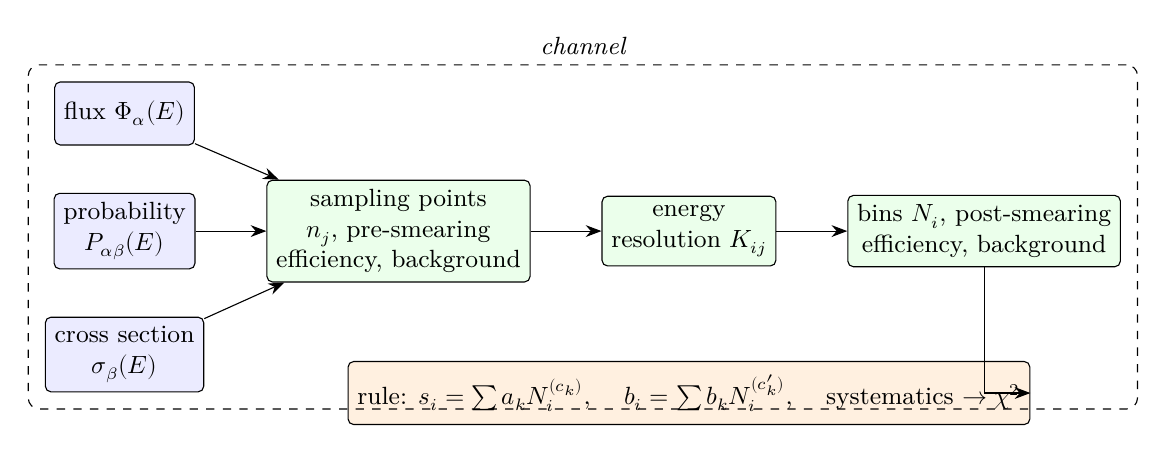
\begin{tikzpicture}[node distance=6mm and 9mm,
  box/.style={draw,rounded corners=2pt,minimum height=8mm,align=center,font=\small,fill=#1},
  box/.default=white, >={Stealth[length=2mm]}]
\node[box=blue!8] (flux) {flux $\Phi_\alpha(E)$};
\node[box=blue!8,below=of flux] (prob) {probability\\$P_{\alpha\beta}(E)$};
\node[box=blue!8,below=of prob] (xs) {cross section\\$\sigma_\beta(E)$};
\node[box=green!8,right=of prob] (pre) {sampling points\\$n_j$, pre-smearing\\efficiency, background};
\node[box=green!8,right=of pre] (smear) {energy\\resolution $K_{ij}$};
\node[box=green!8,right=of smear] (post) {bins $N_i$, post-smearing\\efficiency, background};
\node[box=orange!12,below=12mm of smear] (rule) {rule: $s_i=\sum a_kN^{(c_k)}_i$, \quad $b_i=\sum b_kN^{(c'_k)}_i$, \quad systematics $\to\chi^2$};
\draw[->] (flux) -- (pre); \draw[->] (prob) -- (pre); \draw[->] (xs) -- (pre);
\draw[->] (pre) -- (smear); \draw[->] (smear) -- (post); \draw[->] (post) |- (rule);
\node[draw,dashed,rounded corners,fit=(flux)(xs)(pre)(post),inner sep=6pt,
  label={[font=\small\itshape]above:channel}] {};
\end{tikzpicture}
\caption{How GLoBES computes event rates. A \emph{channel} turns the flux of
one neutrino flavour into events of one flavour in the detector, binned in
reconstructed energy; a \emph{rule} combines channels into signal and
background and computes $\chi^2$.}
\label{fig:channel}
\end{figure}

GLoBES computes events in two energy grids: the \emph{sampling points} $E_j$
(with widths $\Delta E_j$) in true neutrino energy, and the \emph{bins} $i$ in
reconstructed energy (with edges $E_i^\pm$, centres $E_i$ and widths $\Delta
E_i$). A \emph{channel} describes neutrinos produced as $\nu_\alpha$ (or
$\bar\nu_\alpha$) in a flux, detected as $\nu_\beta$ through a cross section,
with an energy resolution (Figure~\ref{fig:channel}). The number of events of
channel $c$ at sampling point $j$ is
\begin{equation}
n_{c,j} = \Phi_\alpha(E_j)\,P(\nu_\alpha\to\nu_\beta;E_j)\,\sigma_\beta(E_j)\,M\,
          \epsilon^\text{pre}_{c,j}\,\Delta E_j + B^\text{pre}_{c,j},
\label{eq:presmear}
\end{equation}
with the detector mass $M$ and the pre-smearing efficiencies and backgrounds
$\epsilon^\text{pre}$ (default 1) and $B^\text{pre}$ (default 0). The flux at
the detector is
\begin{equation}
\Phi_\alpha(E) = \frac{\mathcal N}{L^2}\;\texttt{@norm}\times\texttt{@power}\times
  \texttt{@stored\_muons}\times\texttt{@time}\;\phi_\alpha(E),
\label{eq:flux}
\end{equation}
where $\phi_\alpha$ is the flux table of the AEDL file (or a built-in flux),
normalised to a distance of 1~km, and $\mathcal N$ a constant that depends on
the kind of flux (Section~\ref{sec:aedl-flux}). The cross section $\sigma_\beta(E)
= E\,(\sigma/E)_\beta(E)$ is in $10^{-38}\,\mathrm{cm}^2$ per nucleon. Channels
whose flavours are prefixed with \code{NOSC\_} in AEDL do not oscillate:
$P=\delta_{\alpha\beta}$.

The energy resolution maps the sampling points to the bins,
\begin{equation}
N_{c,i} = \epsilon^\text{post}_{c,i}\sum_j K^{(c)}_{ij}\,n_{c,j} + B^\text{post}_{c,i},
\label{eq:postsmear}
\end{equation}
with the smearing matrix $K_{ij}$, the probability that an event at sampling
point $j$ is reconstructed in bin $i$ (Section~\ref{sec:smearing}), and
post-smearing efficiencies and backgrounds.

\paragraph{Rules.} A rule adds channels with coefficients to a signal and a
background,
\begin{equation}
s_i = \sum_k a_k\,N_{c_k,i},\qquad b_i = \sum_k b_k\,N_{c'_k,i},
\label{eq:rule}
\end{equation}
and the prediction without systematics is $s_i + \beta_0 b_i$ with the
background normalisation $\beta_0$ given by \code{@backgroundcenter}. Only the
bins in the energy window of the rule enter its $\chi^2$.

\section{Getting event rates}

\begin{apifun}{event\_rates(e; rule=1)\\
event\_rates(e, params::OscParams; rule=1)}
The rates of one rule in each bin: of the simulated data, or as predicted for
\code{params}. Returns a named tuple \code{(energy, width, signal, background,
total)}: bin centres and widths, $s_i$, $\beta_0b_i$, and
$s_i+\beta_0b_i$ inside the energy window (zero outside). \code{rule} is a
number or the name of the rule in the AEDL file.
\end{apifun}
\begin{apifun}{total\_events(e; rule=1)\qquad total\_events(e, params; rule=1)}
The sum of \code{event\_rates(...).total}.
\end{apifun}
\begin{apifun}{channel\_rates(e, channel; smeared=true)}
The simulated $N_{c,i}$ of a channel per bin, or with \code{smeared=false}
$n_{c,j}$ per sampling point.
\end{apifun}
\begin{apifun}{rule\_names(e)\qquad channel\_names(e)\qquad bin\_centers(e)\qquad bin\_widths(e)\qquad energy\_range(e)}
Names of rules and channels as in the AEDL file (without \code{\#}), and the
reconstructed energy binning.
\end{apifun}
\begin{apifun}{energy\_window(e; rule=1)\qquad energy\_window!(e, emin, emax; rule=:all)\qquad energy\_window\_bins(e; rule=1)}
The energy window of a rule in GeV, changing it, and the bins inside it.
\end{apifun}

\noindent For example, the spectra of Figure~\ref{fig:nova-rates} come from
\begin{julia}
nova = Experiment("NOvA.glb")
simulate!(truth)
r  = event_rates(nova; rule="Nu_E_Appearance")
io = event_rates(nova, OscParams(truth; Δm31=-truth.Δm31 + truth.Δm21); rule=1)
r.energy, r.signal, r.background, sum(r.total), sum(io.total)
\end{julia}

\begin{figure}[t]
\centering
\begin{tikzpicture}
\begin{axis}[manual,xlabel={$E_\text{rec}$ [GeV]},ylabel={events per bin},xmin=1,xmax=3.5,ymin=0,
  title={\small $\numu\to\nue$ appearance},legend pos=north east,ybar stacked,bar width=0.08,
  every axis plot/.append style={line width=0.3pt}]
\addplot[fill=blue!35,draw=blue!50!black] table[x=E,y=signal]{figures/data/nova_app.dat};
\addplot[fill=gray!40,draw=gray] table[x=E,y=bg]{figures/data/nova_app.dat};
\legend{signal,background}
\end{axis}
\end{tikzpicture}\hfill
\begin{tikzpicture}
\begin{axis}[manual,xlabel={$E_\text{rec}$ [GeV]},ylabel={events per bin},xmin=1,xmax=3.5,ymin=0,
  title={\small total, three hypotheses},legend pos=north east]
\addplot+[const plot mark mid,mark=none] table[x=E,y=total]{figures/data/nova_app.dat};
\addplot+[const plot mark mid,mark=none] table[x=E,y=total_d90]{figures/data/nova_app.dat};
\addplot+[const plot mark mid,mark=none] table[x=E,y=total_io]{figures/data/nova_app.dat};
\legend{true ($\dcp=3\pi/2$),$\dcp=\pi/2$,inverted}
\end{axis}
\end{tikzpicture}
\caption{The $\nue$ appearance rule of \file{NOvA.glb}. Left: signal and
background of the simulated data. Right: the total rates for the true
parameters, for $\dcp=\pi/2$, and for inverted ordering
($\dm{31}\to-\dm{31}+\dm{21}$). Parameters as in Figure~\ref{fig:prob}.}
\label{fig:nova-rates}
\end{figure}

\section{Energy resolution}\label{sec:smearing}

\begin{figure}[t]
\centering
\begin{tikzpicture}
\begin{axis}[wide,height=0.36\linewidth,xlabel={$E$ [GeV]},ylabel={events per GeV},xmin=0,xmax=1.6,ymin=0,
  legend pos=north east]
\addplot[blue!70!black,const plot mark mid] table[x=E,y=rate]{figures/data/smear_pre.dat};
\addplot[red!70!black,const plot mark mid] table[x=E,y=rate]{figures/data/smear_post.dat};
\legend{true energy (sampling points),reconstructed energy (bins)}
\end{axis}
\end{tikzpicture}
\caption{The $\nue$ appearance signal channel of \file{T2K.glb} before and
after the energy resolution, $\sigma_E = 85\,\mathrm{MeV}$. Rates are divided
by the widths of sampling points and bins. Computed with
\code{channel\_rates(t2k, "nu\_e\_signal"; smeared=false)} and
\code{channel\_rates(t2k, "nu\_e\_signal")}.}
\label{fig:smearing}
\end{figure}

The energy resolution of a channel is either given as a matrix in the AEDL
file or computed from a resolution function (Section~\ref{sec:aedl-energy}).
For a Gaussian resolution with width $\sigma(E)$, the element $K_{ij}$ is the
probability that an event with true energy $E_j$ is reconstructed in bin $i$,
\begin{equation}
K_{ij} = \frac12\left[\mathrm{erf}\!\left(\frac{E^+_i-E_j}{\sqrt2\,\sigma(E_j)}\right)
                   -\mathrm{erf}\!\left(\frac{E^-_i-E_j}{\sqrt2\,\sigma(E_j)}\right)\right],
\label{eq:smear}
\end{equation}
rounded to multiples of $10^{-7}$, so that the matrix is sparse. The built-in
resolution functions are
\begin{align}
\texttt{\#standard:}\quad & \sigma(E) = a\,E + b\sqrt{E} + c, \qquad \texttt{@sigma\_e = \{a, b, c\}},\\
\texttt{\#inverse\_beta:}\quad & \sigma(E) = \alpha\sqrt{E/\mathrm{MeV} - 0.8}\;\mathrm{MeV}, \qquad \texttt{@sigma\_e = \{α\}},
\end{align}
the second for reactor antineutrinos detected by inverse beta decay, whose
visible energy is $E-0.8\,\mathrm{MeV}$ (it is $\alpha\,$keV below $1.8\,$MeV).
With the low-pass filter (Section~\ref{sec:filter}) and \code{@type = 2}, the
width is reduced to $\sqrt{\sigma(E)^2-\sigma_f^2}$, since the filter already
averages over $\sigma_f$. Figure~\ref{fig:smearing} shows a spectrum before and
after smearing.

Events whose reconstructed energy falls outside the bins are lost. The
sampling points should therefore extend beyond the bins by a few $\sigma$
(\code{\$sampling\_min}, \code{\$sampling\_max}); by default they coincide with
the bins.

\chapter{\texorpdfstring{$\chi^2$}{chi2} with systematics}\label{ch:chi2}

\section{The Poisson \texorpdfstring{$\chi^2$}{chi2}}\label{sec:poisson}

GLoBES compares the simulated event numbers $n_i$ (the ``data'', from
\code{simulate!}) with the event numbers $N_i$ predicted for a hypothesis with
the Poisson log-likelihood ratio
\begin{equation}
\chi^2 = \sum_i \chi^2_\text{P}(n_i, N_i),\qquad
\chi^2_\text{P}(n, N) = 2\Bigl(N - n + n\ln\frac{n}{N}\Bigr),
\label{eq:poisson}
\end{equation}
which is $-2\ln$ of the ratio of the Poisson probabilities of $n$ for the
predicted mean $N$ and for the best possible mean $n$. For large event numbers,
$\chi^2_\text{P}\to(n-N)^2/n$, the Gaussian $\chi^2$
(Figure~\ref{fig:poisson}). The function is also available as
\code{poisson\_chi2(n, N)}, for user-defined $\chi^2$ functions.

\begin{figure}[t]
\centering
\begin{tikzpicture}
\begin{axis}[wide,height=0.36\linewidth,xlabel={predicted events $N$},ylabel={$\chi^2_\text{P}(n,N)$},
  xmin=0,xmax=25,ymin=0,ymax=20,legend pos=north east]
\addplot table[x=fit,y=n0]{figures/data/poisson.dat};
\addplot table[x=fit,y=n1]{figures/data/poisson.dat};
\addplot table[x=fit,y=n5]{figures/data/poisson.dat};
\addplot table[x=fit,y=n10]{figures/data/poisson.dat};
\addplot[black,dashed] table[x=fit,y=gauss10]{figures/data/poisson.dat};
\legend{$n=0$,$n=1$,$n=5$,$n=10$,$(N-10)^2/10$}
\end{axis}
\end{tikzpicture}
\caption{The Poisson $\chi^2$ of one bin with $n$ observed (simulated) events
as a function of the prediction $N$, and the Gaussian approximation for
$n=10$.}
\label{fig:poisson}
\end{figure}

\paragraph{Empty bins and vanishing predictions.} For $n=0$,
$\chi^2_\text{P}=2N$; an empty bin with $N=0$ contributes nothing. If
systematics push the prediction to $N\le0$ while $n>0$, the logarithm diverges.
Below $N_0=10^{-10}$, $\chi^2_\text{P}$ is therefore continued by its Taylor
expansion of second order around $N_0$, a steep but finite and smooth wall that
minimisers can handle:
\begin{equation}
\chi^2_\text{P}(n, N) = \chi^2_\text{P}(n,N_0) + 2\Bigl(1-\frac{n}{N_0}\Bigr)(N-N_0)
  + \frac{n}{N_0^2}(N-N_0)^2 \qquad (N<N_0).
\end{equation}
A negative prediction for an empty bin gives $2|N|$.

\begin{cdiff}
C GLoBES returns $10^{100}$ for every bin with $N\le0$, including empty bins
with $n=N=0$. A rule with an empty bin (for instance a background that
vanishes at some energies) then has $\chi^2=10^{100}$ whatever the parameters,
and minimisers see a discontinuous function
(Section~\ref{sec:cdiff-poisson}).
\end{cdiff}

\section{Systematics and the pull method}\label{sec:pull}

Systematic uncertainties are described by nuisance parameters $\zeta_k$ (the
``pulls''): for example, the signal normalisation is $(1+\zeta_1)$ times the
nominal one, with a Gaussian uncertainty $\sigma_1$. The $\chi^2$ of a rule is
minimised over them,
\begin{equation}
\chi^2_\text{rule} = \min_{\zeta}\Bigl[\sum_{i\in\text{window}}\chi^2_\text{P}\bigl(n_i,N_i(\zeta)\bigr)
  + \sum_k\frac{(\zeta_k-\zeta_k^0)^2}{\sigma_k^2}\Bigr],
\label{eq:pull}
\end{equation}
independently for every rule~\cite{Fogli:2002pt}, and the $\chi^2$ of an
experiment is the sum over its rules. The minimisation uses Powell's method
(Section~\ref{sec:minimizer}).

\subsection{Built-in systematics functions}\label{sec:builtin-chi2}

Each rule uses one $\chi^2$ function with systematics on and one with
systematics off (\code{@sys\_on\_function} and \code{@sys\_off\_function} in
AEDL). The built-in functions are listed in Table~\ref{tab:chi2functions}.
They use the signal $s_i$ and background $b_i$ of Eq.~\eqref{eq:rule}, the
background normalisation $\beta_0$ and background tilt centre $\tau_0$ of
\code{@backgroundcenter} (default $1:0$), and the errors
$\sigma_1,\dots,\sigma_4$ (\code{@signalerror} $=\sigma_1:\sigma_2$,
\code{@backgrounderror} $=\sigma_3:\sigma_4$, or \code{@sys\_on\_errors}).
With $\bar E = (E_\text{min}+E_\text{max})/2$ and
$\Delta E = E_\text{max}-E_\text{min}$ the reconstructed energy range of the
experiment, and $E_i$ the bin centres:

\begin{table}[t]
\centering\small
\begin{tabularx}{\linewidth}{llcX}
\toprule
Name & Parameters & Old \code{errordim} & Description \\
\midrule
\code{chiSpectrumTilt}    & 4 & 0 & normalisation and tilt of signal and background, Eq.~\eqref{eq:tilt} \\
\code{chiNoSysSpectrum}   & 0 & 2 & spectrum without systematics \\
\code{chiTotalRatesTilt}  & 4 & 4 & as \code{chiSpectrumTilt}, total rates only \\
\code{chiSpectrumOnly}    & 1 & 7 & spectrum with free signal normalisation \\
\code{chiNoSysTotalRates} & 0 & 8 & total rates without systematics \\
\code{chiSpectrumCalib}   & 4 & 9 & normalisation and energy calibration, Eq.~\eqref{eq:calib} \\
\code{chiZero}            & 0 & -- & always 0 (rules used by other rules' $\chi^2$) \\
\bottomrule
\end{tabularx}
\caption{Built-in $\chi^2$ functions. The old \code{errordim} numbers of GLoBES
2.x are still accepted in AEDL (\code{@errordim\_sys\_on}).}
\label{tab:chi2functions}
\end{table}

\paragraph{\code{chiSpectrumTilt}} (four nuisance parameters):
\begin{gather}
N_i = (1+\zeta_1)\,s_i + \frac{\zeta_2}{\Delta E}(E_i-\bar E)\,s_i
    + \beta_0(1+\zeta_3)\,b_i + \frac{\zeta_4}{\Delta E}(E_i-\bar E)\,b_i,
\label{eq:tilt}\\
\chi^2 = \sum_i\chi^2_\text{P}(n_i,N_i) + \frac{\zeta_1^2}{\sigma_1^2} + \frac{\zeta_2^2}{\sigma_2^2}
  + \frac{\beta_0^2\zeta_3^2}{\sigma_3^2} + \frac{(\zeta_4-\tau_0)^2}{\sigma_4^2}.
\end{gather}
The ``tilt'' $\zeta_2$ is a linear distortion of the spectrum, a simple model of
an energy calibration uncertainty.

\paragraph{\code{chiTotalRatesTilt}:} the same $N_i$ and priors, but with
$\chi^2_\text{P}(\sum_i n_i,\sum_i N_i)$, so that only the total number of
events is used.

\paragraph{\code{chiNoSysSpectrum}, \code{chiNoSysTotalRates}:}
$N_i = s_i+\beta_0 b_i$ without nuisance parameters, binned or total.

\paragraph{\code{chiSpectrumOnly}:} $N_i = (1+\zeta_1)s_i + \beta_0b_i$ with no prior
on $\zeta_1$: only the shape of the spectrum is used.

\paragraph{\code{chiSpectrumCalib}} (energy calibration error):
\begin{gather}
N_i = (1+\zeta_1)\,\mathcal S_{\zeta_2}[s]_i + \beta_0(1+\zeta_3)\,\mathcal S_{\tau_0+\zeta_4}[b]_i,
\label{eq:calib}\\
\chi^2 = \sum_i\chi^2_\text{P}(n_i,N_i) + \frac{\zeta_1^2}{\sigma_1^2} + \frac{\zeta_2^2}{\sigma_2^2}
  + \frac{\beta_0^2\zeta_3^2}{\sigma_3^2} + \frac{\zeta_4^2}{\sigma_4^2},
\end{gather}
where $\mathcal S_b$ shifts the energy scale of a spectrum by a relative amount
$b$ (Section~\ref{sec:escale}).

\begin{cdiff}
In \code{chiSpectrumTilt} and \code{chiTotalRatesTilt} C GLoBES applies the
prior of the background tilt to $\zeta_4/\Delta E$ instead of $\zeta_4$, so that
the background tilt error is effectively $\sigma_4\,\Delta E$ instead of
$\sigma_4$ (Section~\ref{sec:cdiff-tilt}).
\end{cdiff}

\subsection{The energy calibration error}\label{sec:escale}

An energy scale error $b$ means that an event reconstructed at energy $E$ in
the simulation is reconstructed at $(1+b)E$ in the real detector, or,
equivalently, that the bin $[E_i^-,E_i^+]$ of the shifted spectrum contains the
events of the nominal spectrum between $(1+b)E_i^-$ and $(1+b)E_i^+$. With the
cumulative event number $F(E)$ of the nominal spectrum, which is known at the
bin edges,
\begin{equation}
F(E_i^+) = \sum_{k\le i} s_k ,\qquad
\mathcal S_b[s]_i = F\bigl((1+b)E_i^+\bigr) - F\bigl((1+b)E_i^-\bigr).
\label{eq:shift}
\end{equation}
Between the edges, $F$ is interpolated with a monotone cubic Hermite
interpolant (Fritsch--Carlson with the Fritsch--Butland slopes~\cite{Fritsch:1980}
and shape-preserving one-sided slopes at the ends). There are no events outside
the binned range: $F$ is $0$ below it and constant above it. As a result,
$\mathcal S_b$
\begin{itemize}
\item reproduces the spectrum for $b=0$ and conserves the number of events
      inside the range,
\item never gives negative rates, because $F$ is monotone,
\item is smooth in $b$, so that the minimisation over $b$ is well behaved,
\item works for bins of any width.
\end{itemize}
\code{energy\_scale\_shift(e, rates, b)} applies it to any spectrum of an
experiment.

\begin{figure}[t]
\centering
\begin{tikzpicture}
\begin{axis}[manual,xlabel={$E_\text{rec}$ [GeV]},ylabel={events per bin},xmin=1,xmax=3.5,ymin=0,
  title={\small $b=\pm5\%$},legend pos=north west]
\addplot[black,const plot mark mid] table[x=E,y=nominal]{figures/data/escale_spec.dat};
\addplot[blue!70!black,const plot mark mid] table[x=E,y=jl_p]{figures/data/escale_spec.dat};
\addplot[blue!70!black,const plot mark mid,dashed] table[x=E,y=jl_m]{figures/data/escale_spec.dat};
\addplot[red!70!black,only marks,mark=o,mark size=1.2pt] table[x=E,y=c_p]{figures/data/escale_spec.dat};
\addplot[red!70!black,only marks,mark=x,mark size=1.6pt] table[x=E,y=c_m]{figures/data/escale_spec.dat};
\legend{$b=0$,$b=+0.05$,$b=-0.05$,C $+0.05$,C $-0.05$}
\end{axis}
\end{tikzpicture}\hfill
\begin{tikzpicture}
\begin{axis}[manual,xlabel={$b$},ylabel={$\chi^2$},xmin=-0.01,xmax=0.01,ymin=0,
  title={\small $\chi^2$ of the shifted spectrum},legend pos=north east,
  xticklabel style={/pgf/number format/fixed}, scaled x ticks=false]
\addplot table[x=b,y=jl]{figures/data/escale_chi.dat};
\addplot table[x=b,y=c]{figures/data/escale_chi.dat};
\legend{GLoBES.jl,C GLoBES}
\end{axis}
\end{tikzpicture}
\caption{The energy scale shift applied to the $\numu$ disappearance signal of
\file{NOvA.glb}. Left: the spectrum shifted by $\pm5\%$ with
Eq.~\eqref{eq:shift} (lines) and with the method of C GLoBES (symbols).
Right: $\chi^2_\text{P}$ of the shifted against the nominal spectrum. The
interpolation of C GLoBES makes it kinked at $b=0$; Eq.~\eqref{eq:shift} is
smooth with a minimum at $b=0$.}
\label{fig:escale}
\end{figure}

\begin{cdiff}
C GLoBES computes $\mathcal S_b[s]_i = (1+b)\,s(\delta_i)$ by linear
interpolation of the rates at the shifted bin positions
$\delta_i = b(i+t_0+\frac12)+i$. Interpolating the rates and not their
integral makes $\chi^2$ kinked at $b=0$ in every bin (Figure~\ref{fig:escale}),
the last bin is counted twice when the spectrum is shifted past the upper end,
and the method requires equal bins. See Section~\ref{sec:cdiff-escale}.
\end{cdiff}

\section{Computing \texorpdfstring{$\chi^2$}{chi2}}

\begin{apifun}{chi2(test::OscParams; experiment=:all, rule=:all, systematics=true, setup=current\_setup())}
$\chi^2$ of the hypothesis \code{test}, minimised over the systematics of
every rule but not over oscillation parameters, summed over all experiments
and rules, or for one experiment (an \code{Experiment}) or one rule (a number
or name; with \code{experiment=:all} the rule number in every experiment).
\code{systematics=false} uses the \code{@sys\_off\_function} of the rules.
\end{apifun}
\begin{apifun}{systematics!(e, on::Bool; rule=:all)\qquad systematics!(on::Bool; setup)}
Switch systematics on or off, for some rules or for all experiments.
\end{apifun}
\begin{apifun}{chi2\_function(e; rule=1, systematics=true)\\
chi2\_function!(e, name; rule=:all, errors, systematics=true)}
The name of the $\chi^2$ function of a rule, and changing it, with the errors
of its nuisance parameters.
\end{apifun}
\begin{apifun}{systematic\_errors(e; rule=1, systematics=true)\\
systematic\_errors!(e, errors; rule=:all, systematics=true)}
The prior widths $\sigma_k$ of the nuisance parameters.
\end{apifun}

\begin{julia}
chi2(test)                                   # all experiments and rules
chi2(test; experiment=nova, rule="Nu_E_Appearance")
chi2(test; systematics=false)                # statistics only
chi2_function!(nova, "chiSpectrumCalib"; rule=2, errors=[0.025, 0.02, 0.05, 0.02])
systematic_errors!(nova, [0.05, 0.0001, 0.1, 0.0001]; rule=1)
\end{julia}

\section{User-defined systematics\texorpdfstring{$^\ast$}{*}}\label{sec:userchi2}

A $\chi^2$ function that is not built in, for example for systematics that are
correlated between rules or between a near and a far detector, is defined with
\begin{apifun}{define\_chi2(f, name, n\_params; setup=current\_setup())}
Register \code{f(e::Experiment, rule::Int, x, errors) -> χ²} under
\code{name}. \code{x} are the \code{n\_params} nuisance parameters, which are
minimised over, and \code{errors} their prior widths from the AEDL file or
\code{chi2\_function!}. \code{f} must include the priors.
\end{apifun}

\noindent Inside \code{f}, \code{true\_rates(e; rule)} are the simulated rates
$n_i$ of a rule and \code{fit\_rates(e; rule)} the signal $s_i$ and background
$b_i$ predicted for the parameters being tested (before $\beta_0$ and
systematics), \code{energy\_window\_bins(e; rule)} the bins to sum over, and
\code{energy\_scale\_shift} and \code{poisson\_chi2} help with the
computation. The functions must be defined before AEDL files that use them are
loaded. For example, a normalisation error common to the signal and background:
\begin{julia}
define_chi2("chiCommonNorm", 1) do e, rule, x, errors
    n = true_rates(e; rule)
    s, b = fit_rates(e; rule)
    β0 = e.data.rules[rule].bg_centers[1]
    sum(poisson_chi2(n[i], (1 + x[1]) * (s[i] + β0 * b[i])) for i in energy_window_bins(e; rule)) +
        (x[1] / errors[1])^2
end
nova = Experiment("NOvA.glb")
chi2_function!(nova, "chiCommonNorm"; errors=[0.05])
\end{julia}
A rule whose events enter the $\chi^2$ of another rule (a near detector, say)
uses \code{chiZero}; the function of the other rule reads its rates with
\code{true\_rates} and \code{fit\_rates}. For correlations between
experiments, \code{experiments()} gives all experiments of the setup.

\chapter{Correlations, projections and degeneracies}\label{ch:fits}

\section{Projections}

The $\chi^2$ of Chapter~\ref{ch:chi2} tests one point of parameter space. To
measure one parameter, say $\theta_{13}$, all the others must be allowed to
take the values that fit the data best, since they are not known exactly and
can mimic a different $\theta_{13}$. This is the \emph{projection} of the
$\chi^2$ onto the $\theta_{13}$ axis (or \emph{profiling}, or
\emph{marginalisation}):
\begin{equation}
\chi^2(\theta_{13}) = \min_{\theta_{12},\theta_{23},\dcp,\dm{21},\dm{31},\rho}
  \Bigl[\chi^2(\theta_{12},\theta_{13},\dots,\rho) + \chi^2_\text{prior}\Bigr].
\label{eq:projection}
\end{equation}
More generally, any set of parameters can be kept fixed and the others
minimised over. The $\chi^2$ of a projection onto $k$ parameters is
distributed as $\chi^2$ with $k$ degrees of freedom; Table~\ref{tab:cl} gives
the values for the usual confidence levels.

\begin{table}[t]
\centering\small
\begin{tabular}{lccccc}
\toprule
& $1\sigma$ (68.27\%) & 90\% & $2\sigma$ (95.45\%) & 99\% & $3\sigma$ (99.73\%) \\
\midrule
1 d.o.f. & 1.00 & 2.71 & 4.00 & 6.63 & 9.00 \\
2 d.o.f. & 2.30 & 4.61 & 6.18 & 9.21 & 11.83 \\
3 d.o.f. & 3.53 & 6.25 & 8.02 & 11.34 & 14.16 \\
\bottomrule
\end{tabular}
\caption{$\Delta\chi^2$ for confidence levels and 1--3 parameters (degrees of
freedom).}
\label{tab:cl}
\end{table}

\section{External information: priors}\label{sec:priors}

Parameters that an experiment does not measure well (like the solar
parameters for a long-baseline experiment) or the matter density are
constrained by external information, as Gaussian priors:
\begin{equation}
\chi^2_\text{prior} = \sum_{k\ \text{free}}\frac{(x_k-\hat x_k)^2}{\sigma_k^2}
  + \sum_{e\ \text{free}}\frac{(\rho_e-\hat\rho_e)^2}{\sigma_\rho^2},
\label{eq:prior}
\end{equation}
summed over the fitted parameters. The centres $\hat x_k$ are the simulated
(true) values unless given otherwise; parameters without $\sigma_k$ have no
prior. Any other prior is added as a function of the parameters.

\section{Fitting}

\begin{apifun}{marginalize(start::OscParams; free, fixed, priors=(;), centers=simulated\_params(),\\
\phantom{marginalize(}prior=nothing, experiment=:all, setup=current\_setup()) -> FitResult}
Minimise $\chi^2+\chi^2_\text{prior}$ over the parameters listed in
\code{free} (or over all except those in \code{fixed}; by default over all),
starting at \code{start}, with the fixed parameters at their values in
\code{start}. Parameter names are those of Table~\ref{tab:params} and
\code{:ρ} for the matter densities of all experiments.
\code{priors} are the $\sigma_k$ as a named tuple, \code{centers} the
$\hat x_k$, and \code{prior} a function \code{OscParams -> Float64} added to
$\chi^2$. The result has the fields \code{chi2}, \code{params} (the parameters
at the minimum), \code{free} and \code{iterations} (the number of $\chi^2$
evaluations).
\end{apifun}

\begin{julia}
test = with_param(truth, :sin²2θ13, 0.08)
r = marginalize(test; fixed=(:θ13,),
                priors=(θ12=0.03truth.θ12, Δm21=0.03truth.Δm21, ρ=0.05))
r.chi2, r.params.δ, r.params.ρ

# only δ and the density free, a non-Gaussian prior on θ23
marginalize(test; free=(:δ, :ρ), priors=(ρ=0.05,),
            prior = p -> p.sin²θ23 < 0.5 ? 0.0 : 4.0)
\end{julia}

\begin{note}
The minimiser finds the minimum nearest to \code{start} (a local minimum).
Start fits at the true parameters, or, to find degeneracies, at the points
where they are expected (Section~\ref{sec:degeneracies}).
\end{note}

\section{Scans}

\begin{apifun}{chi2\_scan(base, x => xs; kwargs...) -> Vector\\
chi2\_scan(base, x => xs, y => ys; kwargs...) -> Matrix}
$\chi^2$ on a grid of one or two parameters, with all others as in
\code{base}. The parameter names include the derived ones of
Table~\ref{tab:params}, such as \code{:sin²2θ13}. Without keyword arguments,
each point is \code{chi2}; with any of the keywords of \code{marginalize},
each point is minimised over the other parameters, the scanned ones fixed.
The matrix has one row per value of \code{x}.
\end{apifun}

\noindent Figure~\ref{fig:delta} shows the projection onto $\dcp$ for NOvA,
Figure~\ref{fig:contours} a two-parameter scan for T2K and NOvA together:
\begin{julia}
δs = range(0, 2π, 73)
sys = chi2_scan(truth, :δ => δs)                                   # systematics only
fit = chi2_scan(truth, :δ => δs; free=(:θ23, :Δm31, :ρ), priors=(ρ=0.05,))
grid = chi2_scan(truth, :sin²2θ13 => range(0.06, 0.115, 56), :δ => δs)
\end{julia}

\begin{figure}[t]
\centering
\begin{tikzpicture}
\begin{axis}[wide,height=0.4\linewidth,xlabel={$\dcp/\pi$},ylabel={$\Delta\chi^2$},xmin=0,xmax=2,ymin=0,
  legend pos=north west,legend columns=1]
\addplot table[x=delta,y=sys]{figures/data/nova_delta.dat};
\addplot table[x=delta,y=fit]{figures/data/nova_delta.dat};
\addplot table[x=delta,y=fit_io]{figures/data/nova_delta.dat};
\addplot[gray,thin,dashed,domain=0:2] {1}; \addplot[gray,thin,dashed,domain=0:2] {4};
\addplot[gray,thin,dashed,domain=0:2] {9};
\legend{systematics only,fit of $\theta_{23}$\,$\dm{31}$\,$\rho$ (normal),fit started at inverted ordering}
\end{axis}
\end{tikzpicture}
\caption{$\Delta\chi^2$ as a function of the tested $\dcp$ for \file{NOvA.glb},
true $\dcp=3\pi/2$ and normal ordering: with all other parameters fixed at the
true values, minimised over $\theta_{23}$, $\dm{31}$ and $\rho$ (5\% prior),
and the same fit started at $\dm{31}\to-\dm{31}+\dm{21}$, which finds the
best fit with inverted ordering (the sign degeneracy). Dashed lines: $1$, $2$
and $3\sigma$ for one parameter.}
\label{fig:delta}
\end{figure}

\begin{figure}[t]
\centering
\begin{tikzpicture}
\begin{axis}[wide,height=0.45\linewidth,xlabel={$\sst{13}$},ylabel={$\dcp/\pi$},xmin=0.06,xmax=0.115,
  ymin=0,ymax=2,legend pos=north east,
  xticklabel style={/pgf/number format/fixed,/pgf/number format/precision=3},scaled x ticks=false]
\addplot[blue!70!black,thick] table[x=x,y=y]{figures/data/t2k_nova_1s.dat};
\addplot[red!70!black,thick] table[x=x,y=y]{figures/data/t2k_nova_2s.dat};
\addplot[green!50!black,thick] table[x=x,y=y]{figures/data/t2k_nova_3s.dat};
\addplot[only marks,mark=*,mark size=1.5pt,black] coordinates {(0.086064,1.5)};
\legend{$1\sigma$,$2\sigma$,$3\sigma$}
\end{axis}
\end{tikzpicture}
\caption{Allowed regions (2 degrees of freedom) in the $\sst{13}$--$\dcp$
plane for T2K and NOvA together, systematics only (\code{chi2\_scan} with two
parameters on a $56\times73$ grid). The dot marks the true values.}
\label{fig:contours}
\end{figure}

\section{The minimiser}\label{sec:minimizer}

GLoBES minimises with Powell's conjugate direction method and Brent's line
minimisation~\cite{NR}, which needs no derivatives. Two strategies are
available, chosen with \code{minimizer!}:
\begin{description}
\item[\code{:nested}] (default) Powell's method over the free oscillation
  parameters. At every step, the systematics of each rule are minimised
  separately (Eq.~\eqref{eq:pull}), each with its own Powell minimisation.
\item[\code{:hybrid}] One Powell minimisation over the free oscillation
  parameters and all nuisance parameters together, which can be faster with
  many rules.
\end{description}
The tolerances are $10^{-5}$ (relative) for oscillation parameters and
$10^{-8}$ for systematics. Since Powell's method can stop early in narrow
curved valleys, the minimisation over oscillation parameters is restarted with
fresh directions until it no longer improves (at most 10 times).

\begin{cdiff}
C GLoBES writes Powell's test for replacing a direction with a macro
\code{SQR(a)} that stores its argument in a static variable. Used twice in one
expression this is undefined behaviour, and GCC computes a different formula
than intended. C GLoBES also does not restart. Both can make fits stop at
points that are not minima (Section~\ref{sec:cdiff-powell}).
\end{cdiff}

\section{Degeneracies}\label{sec:degeneracies}

The appearance probability depends on $\theta_{13}$, $\dcp$, $\theta_{23}$ and
the sign of $\dm{31}$ in similar ways, so that different parameter sets can
give nearly the same event rates~\cite{Barger:2001yr}:
\begin{itemize}
\item the \emph{intrinsic} ($\theta_{13}$, $\dcp$) degeneracy;
\item the \emph{sign} degeneracy between normal and inverted ordering,
  ($\dm{31}\to-\dm{31}+\dm{21}$);
\item the \emph{octant} degeneracy, $\theta_{23}\to\pi/2-\theta_{23}$.
\end{itemize}
Each gives a local minimum of $\chi^2$. Since the minimiser only finds the
nearest minimum, a degenerate solution is found by starting the fit near it,
as in Figure~\ref{fig:delta}:
\begin{julia}
mirror = OscParams(truth; Δm31=-truth.Δm31 + truth.Δm21, θ23=π/2 - truth.θ23)
deg = marginalize(mirror; priors=(θ12=0.03truth.θ12, Δm21=0.03truth.Δm21, ρ=0.05))
deg.chi2, deg.params
\end{julia}
The projection including degeneracies is the smallest $\chi^2$ of all local
minima. A coarse scan of $\chi^2$ with systematics only (\code{chi2\_scan}) is
a good way to find where to start the fits.

\chapter{Changing experiments at runtime}\label{ch:runtime}

Most properties of an experiment can be changed after it is loaded, for
example to study the sensitivity as a function of the baseline or the running
time. After any change, call \code{simulate!} again so that the simulated data
match the new experiment.

\section{Exposure}\label{sec:exposure}

\begin{apifun}{target\_mass(e)\qquad target\_mass!(e, mass)}
The fiducial detector mass (in the units of the AEDL file, usually kt).
\end{apifun}
\begin{apifun}{running\_time(e; flux=1)\qquad running\_time!(e, years; flux=:all)}
The running time of one flux, or setting it for one or all fluxes.
\end{apifun}
\begin{apifun}{source\_power(e; flux=1)\qquad source\_power!(e, power; flux=:all)}
The source power: beam power, or useful parent decays per year.
\end{apifun}

\noindent Since the event numbers are proportional to all three, a scan over
the exposure is
\begin{julia}
for years in (1, 2, 5, 10)
    running_time!(nova, years / 2)            # half neutrinos, half antineutrinos
    simulate!(truth)
    println(years, "  ", chi2(OscParams(truth; δ=0.5π)))
end
\end{julia}

\section{Baseline and matter profile}

\code{baseline!(e, L)} changes the baseline and recomputes the density profile
as the AEDL file defines it, \code{density\_profile!(e, lengths, densities)}
sets any profile (Section~\ref{sec:profiles}). Note that the flux decreases as
$1/L^2$ when the baseline changes:
\begin{julia}
nf = Experiment("NFstandard.glb")
for L in 1000:1000:8000
    baseline!(nf, L)
    simulate!(truth)
    println(L, "  ", total_events(nf; rule=1))
end
\end{julia}

\section{Systematics and energy windows}

\code{systematics!}, \code{chi2\_function!} and \code{systematic\_errors!}
(Chapter~\ref{ch:chi2}) change the systematics treatment of rules, and
\code{energy\_window!} their energy window.

\section{AEDL variables}

AEDL files can use variables that are defined by the program. They are passed
as keyword arguments when the experiment is loaded; numbers become variables
and vectors become lists:
\begin{julia}
nf = Experiment("NFvar.glb"; BASELINE=3000, emax=50)
\end{julia}
In the AEDL file, they are used like any variable,
\code{\$baseline = BASELINE} (Section~\ref{sec:aedl-variables}). Lists are
named with a leading \code{\%} in AEDL; the keyword is given without it.
This is the way to change things that cannot be changed after loading, such
as the number of bins or the energy range.

\section{The low-pass filter\texorpdfstring{$^\ast$}{*}}

The filter of Section~\ref{sec:filter} is set in AEDL with
\code{\$filter\_state} and \code{\$filter\_value}; at runtime, use
\code{glbSetFilterStateInExperiment(i, GLB\_ON)} and
\code{glbSetFilterInExperiment(i, σ)} with the experiment number
\code{i} (Chapter~\ref{ch:compat}).

\chapter{Non-standard physics}\label{ch:nonstandard}

GLoBES computes event rates from oscillation probabilities, and nothing else
in the simulation depends on how these are computed. To simulate a model
beyond three-flavour oscillations (sterile neutrinos, non-standard
interactions, decoherence, decay, \dots) replace the probability engine.

\begin{apifun}{probability\_engine!(P!, extra; setup=current\_setup())\\
standard\_engine!(; setup=current\_setup())}
Use \code{P!} to compute probabilities, with the additional parameters named
in \code{extra}, or go back to the standard engine. \code{P!(P, params, E,
antineutrino, lengths, densities)} fills the $3\times3$ matrix
\code{P[α, β]} $=P(\nu_\alpha\to\nu_\beta)$ for the \code{OscParams}
\code{params} at energy \code{E} (GeV) through the layers of the matter
profile (km and $\mathrm{g/cm^3}$, already scaled by $\rho$).
\end{apifun}

\noindent After the engine is replaced, \code{OscParams} must have the
additional parameters (\code{extra=(name=value, ...)}), and the data must be
simulated again. The additional parameters work everywhere the standard ones
do: they can be fitted, have priors, and be scanned.

As an example, here is an engine that multiplies the standard probabilities
by $1-\epsilon$, a crude model of neutrino decay or of a loss of
normalisation:
\begin{julia}
engine = GLoBES.StandardEngine()
probability_engine!((:ϵ,)) do P, p, E, anti, lengths, densities
    GLoBES.set_oscillation_parameters!(engine, p.values[1:6])
    GLoBES.probability_matrix!(P, engine, anti ? -1 : +1, E, length(lengths),
                               lengths, densities, -1.0)
    P .*= 1 - p.ϵ
end

truth = OscParams(truth; extra=(ϵ=0.0,))
simulate!(truth)
r = marginalize(OscParams(truth; ϵ=0.1); free=(:ϵ, :θ23), priors=(θ23=0.05,))
r.params.ϵ                     # ≈ 0: the data have no loss
\end{julia}
The standard engine used here (\code{GLoBES.StandardEngine},
\code{GLoBES.set\_oscillation\_parameters!} and
\code{GLoBES.probability\_matrix!}) is the one of Chapter~\ref{ch:prob}: a
model that modifies the Hamiltonian can build on its code in
\file{src/probability.jl}.

\begin{note}
The engine is called for every sampling point of every experiment for every
$\chi^2$ evaluation, so it should be fast and should not allocate memory.
\end{note}


\part{The Abstract Experiment Definition Language}\label{part:aedl}
\chapter{Getting started with AEDL}\label{ch:aedl-intro}

\section{The concept}

An experiment in GLoBES has one neutrino source (a point source, stationary
in time), one baseline with its matter density profile, and one detector. The
detector is described by its response to neutrinos of each flavour: cross
sections, energy resolution, efficiencies and backgrounds. The building blocks
are
\begin{description}
\item[fluxes] (\code{nuflux}) of the source, from a table or built in;
\item[cross sections] (\code{cross}), from tables;
\item[energy resolutions] (\code{energy}), a resolution function or a matrix;
\item[channels] (\code{channel}): one flux, one initial and one final flavour,
  one cross section and one energy resolution, with efficiencies;
\item[rules] (\code{rule}): signal and background, each a weighted sum of
  channels, with a $\chi^2$ function for systematics.
\end{description}
The $\chi^2$ of an experiment is the sum of the $\chi^2$ of its rules, and the
$\chi^2$ of a setup the sum over its experiments (Figure~\ref{fig:concept}).
Chapter~\ref{ch:rates} gives the formulas.

\begin{figure}[t]
\centering
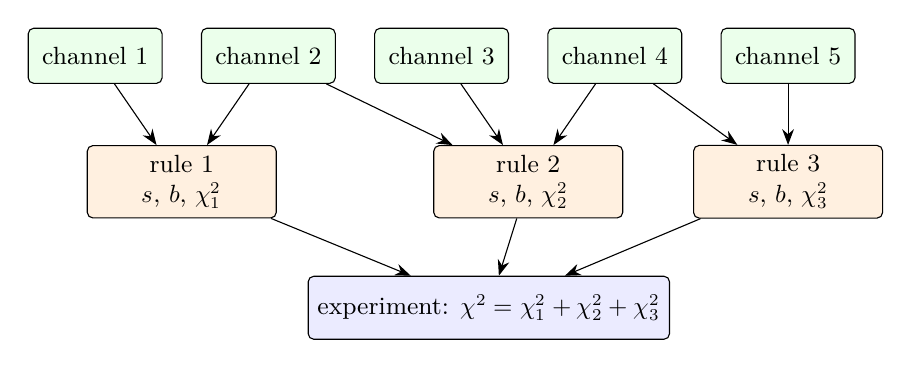
\begin{tikzpicture}[>={Stealth[length=2mm]},font=\small,
  ch/.style={draw,rounded corners=2pt,fill=green!8,minimum width=17mm,minimum height=7mm},
  ru/.style={draw,rounded corners=2pt,fill=orange!12,minimum width=24mm,minimum height=8mm,align=center},
  ex/.style={draw,rounded corners=2pt,fill=blue!8,minimum width=40mm,minimum height=8mm}]
\node[ch] (c1) at (0,0) {channel 1};
\node[ch] (c2) at (2.2,0) {channel 2};
\node[ch] (c3) at (4.4,0) {channel 3};
\node[ch] (c4) at (6.6,0) {channel 4};
\node[ch] (c5) at (8.8,0) {channel 5};
\node[ru] (r1) at (1.1,-1.6) {rule 1\\$s$, $b$, $\chi^2_1$};
\node[ru] (r2) at (5.5,-1.6) {rule 2\\$s$, $b$, $\chi^2_2$};
\node[ru] (r3) at (8.8,-1.6) {rule 3\\$s$, $b$, $\chi^2_3$};
\node[ex] (e) at (5,-3.2) {experiment: $\chi^2=\chi^2_1+\chi^2_2+\chi^2_3$};
\draw[->] (c1) -- (r1); \draw[->] (c2) -- (r1); \draw[->] (c3) -- (r2);
\draw[->] (c4) -- (r2); \draw[->] (c2) -- (r2); \draw[->] (c5) -- (r3); \draw[->] (c4) -- (r3);
\draw[->] (r1) -- (e); \draw[->] (r2) -- (e); \draw[->] (r3) -- (e);
\end{tikzpicture}
\caption{Channels, rules and experiments. A channel can be used in several
rules, as signal in one and as background in another.}
\label{fig:concept}
\end{figure}

\section{A simple example}

The file \file{test/data/Simple.glb} describes a superbeam with a water
Cherenkov detector at 295~km:

\VerbatimInput[breaklines,frame=leftline,framerule=1.5pt,rulecolor=\color{orange!70!black},
  xleftmargin=6pt,framesep=8pt,fontsize=\small,numbers=left,numbersep=4pt]{../../test/data/Simple.glb}

\noindent It defines a flux from a table (lines 9--14), the detector mass, the
energy bins and sampling points (lines 17--26), the baseline and matter
profile (lines 29--30), two cross sections, a Gaussian energy resolution, four
channels, and two rules. The channel \code{\#mu\_e\_eff} has an energy dependent
efficiency computed in AEDL by interpolation (lines 47--53). Loaded with
\begin{julia}
simple = Experiment("Simple.glb")
\end{julia}
it can be used like any other experiment.

\section{Syntax}\label{sec:aedl-syntax}

\paragraph{File structure.} An AEDL file starts with the eight characters
\code{\%!GLoBES}. It should declare the GLoBES version it is written for,
\code{\$version = "3.0.0"}. Comments are as in C, \code{/* ... */} and
\code{// ...} to the end of the line.

\paragraph{Global and local variables.} Variables starting with \code{\$} are
global properties of the experiment (\code{\$baseline = 295}). Variables
starting with \code{@} belong to an environment
(\code{@time = 5} inside \code{nuflux}). Numbers are converted to integers
where integers are expected. Lists are written in braces,
\code{\$densitytab = \{2.8, 3.5\}}.

\paragraph{Environments and names.} Fluxes, cross sections, energy
resolutions, channels and rules are environments,
\begin{aedl}
channel(#name)<
   @channel = ...
>
\end{aedl}
named with a \code{\#}. Names are numbered in the order of their first
appearance within each type (starting at 1 in GLoBES.jl), and must be unique
across all types. A name can be declared before it is defined with an empty
environment, \code{channel(\#later)<>}. \code{rule\_names} and
\code{channel\_names} return the names of an experiment.

\paragraph{User variables and expressions.}\label{sec:aedl-variables}
Variables without prefix are constants for use in expressions:
\begin{aedl}
L = 1300
$baseline = L
$emax = 2 * sqrt(L / 100) + 0.5^2
\end{aedl}
The operators are \code{+ - * / \^}, and the functions \code{sin}, \code{cos},
\code{tan}, \code{asin}, \code{acos}, \code{atan}, \code{log}, \code{log10},
\code{exp} and \code{sqrt}, which apply to every element of a list. Variables
can also be defined by the program: \code{Experiment(file; L=810)}
(Chapter~\ref{ch:runtime}). Lists are stored in variables starting with
\code{\%}, \code{\%effs = \{0.2, 0.4, 0.6\}}.

\paragraph{List functions.}
\begin{description}[style=nextline,leftmargin=3cm]
\item[\code{bincenter()}] the centres of the energy bins defined so far;
\item[\code{samplingbincenter()}] the centres of the sampling points;
\item[\code{interpolation(x, y, k, z)}] the values at \code{z} of the linear
  ($k=1$) or natural cubic spline ($k=2$) interpolation of the points
  $(x, y)$;
\item[\code{copy(l)}] a copy of a list, needed when a list is used twice;
\item[\code{reverse(l)}] the list in reverse order;
\item[\code{echo(x)}, \code{echon(x)}, \code{line(n)}] print values (for
  debugging AEDL files), without or with line feeds, or $n$ line feeds.
\end{description}

\paragraph{Includes and several experiments.} \code{include "file.glb"}
inserts another file (which need not start with \code{\%!GLoBES}); includes
can be nested ten levels deep. Several experiments are separated by
\code{\#NEXT\#}, which resets all names, so that
\begin{aedl}
%!GLoBES
include "NOvA.glb"
#NEXT#
include "T2K.glb"
\end{aedl}
defines two experiments, loaded with \code{load\_experiments}.

\paragraph{Where files are found.} Included files, flux files and cross
section files are looked up in the current directory, in the directory of the
AEDL file that names them, and in the directories of \code{GLB\_PATH}.

\begin{cdiff}
C GLoBES looks for data files only in the current directory and in
\code{GLB\_PATH}, not next to the AEDL file, so that loading an experiment from
another directory fails to find its flux and cross section files.
\end{cdiff}

\chapter{Experiment definition with AEDL}\label{ch:aedl-reference}

This chapter lists all AEDL directives. Defaults are given in brackets.

\section{Source and integrated luminosity}\label{sec:aedl-flux}

\begin{center}\small
\begin{tabularx}{\linewidth}{lX}
\toprule
\multicolumn{2}{l}{\code{nuflux(\#name)< ... >} (or the older \code{flux}, see below)} \\
\midrule
\code{@flux\_file = "file"} & flux table (see below) \\
\code{@builtin = n} & built-in flux: 1 $\mu^+$ decay, 2 $\mu^-$ decay (neutrino factory),
  3 $\beta^+$ decay, 4 $\beta^-$ decay (beta beam) \\
\code{@time} & running time [1] \\
\code{@power} & source power [1], e.g.\ MW \\
\code{@stored\_muons}, \code{@stored\_ions} & useful parent decays per year [1] \\
\code{@norm} & normalisation of the flux table [1] \\
\code{@parent\_energy} & muon energy in GeV (built-in 1, 2) \\
\code{@gamma}, \code{@end\_point} & Lorentz factor of the ions and endpoint of the
  decay in GeV (built-in 3, 4) \\
\midrule
\code{\$target\_mass} & fiducial detector mass, e.g.\ kt \\
\bottomrule
\end{tabularx}
\end{center}

\paragraph{Flux files} have 501 lines of seven columns, with equidistant
energies:
\[
E\ [\mathrm{GeV}]\quad \phi_{\nue}\quad\phi_{\numu}\quad\phi_{\nu_\tau}\quad
\phi_{\bar\nu_e}\quad\phi_{\bar\nu_\mu}\quad\phi_{\bar\nu_\tau}
\]
Lines starting with \code{\#} are comments. The flux is interpolated linearly
and is zero outside the table. Unused flavours must be given as zeros.

\paragraph{Normalisation.} The flux in Eq.~\eqref{eq:flux} is
$\mathcal N/L^2\times$\code{@norm}$\times$\code{@power}$\times$\code{@stored\_muons}$\times$\code{@time}$\times\phi(E)$,
with $\mathcal N=1$ for \code{nuflux} tables. Together with the cross sections
in $10^{-38}\,\mathrm{cm^2}$ per nucleon and the target mass $M$, the number
of events per GeV is
\begin{equation}
\frac{dN}{dE} = \frac{\texttt{@norm}\times\texttt{@power}\times\texttt{@time}\times M}{(L/\mathrm{km})^2}\,
  \phi(E)\,\frac{\sigma(E)}{10^{-38}\,\mathrm{cm}^2}\,P(E).
\end{equation}
If the table gives the number of neutrinos per GeV and per area $A$ at a
distance $L_0$ for an integrated luminosity $\mathcal L$ (in the units
$\mathcal L_u$ chosen for \code{@power}$\times$\code{@time}), the normalisation is
\begin{equation}
\texttt{@norm} = \frac{\mathrm{cm}^2}{A}\left(\frac{L_0}{\mathrm{km}}\right)^2
  \frac{N_\text{target}}{M_u}\times10^{-38}\times\frac{\mathcal L_u}{\mathcal L},
\end{equation}
with $N_\text{target}/M_u$ the number of target nucleons per unit of the
target mass ($6.022\times10^{32}$ per kt). The older environment \code{flux}
multiplies by $\mathcal N = 5.1989$ in addition; replace \code{flux} by
\code{nuflux} and multiply \code{@norm} by $5.1989$ to convert. Built-in fluxes
have their own normalisation and need no \code{@norm}.

\begin{figure}[t]
\centering
\begin{tikzpicture}
\begin{axis}[manual,xlabel={$E$ [GeV]},ylabel={$\phi$ at 1~km [a.u.]},xmin=0,xmax=50,ymin=0,
  title={\small neutrino factory, $\mu^+$, 50 GeV},legend pos=north west]
\addplot table[x=E,y=numubar]{figures/data/nf_flux.dat};
\addplot table[x=E,y=nue]{figures/data/nf_flux.dat};
\legend{$\bar\nu_\mu$,$\nue$}
\end{axis}
\end{tikzpicture}\hfill
\begin{tikzpicture}
\begin{semilogxaxis}[manual,xlabel={$E$ [GeV]},ylabel={$\sigma/E$ [$10^{-38}\,\mathrm{cm^2/GeV}$]},
  xmin=0.1,xmax=100,ymin=0,title={\small charged current, \file{XCC.dat}},legend pos=north west]
\addplot table[x=E,y=numu]{figures/data/xsec.dat};
\addplot table[x=E,y=numubar]{figures/data/xsec.dat};
\legend{$\numu$,$\bar\nu_\mu$}
\end{semilogxaxis}
\end{tikzpicture}
\caption{Left: the built-in neutrino factory flux (\code{@builtin = 1}) of
\file{NFstandard.glb}, \code{flux(nf, E; flavour=:μ, antineutrino=true, L=1)}.
Right: the charged-current cross sections per nucleon divided by energy,
\code{cross\_section(nf, E; flavour=:μ) / E}.}
\label{fig:flux}
\end{figure}

\paragraph{Built-in fluxes.} The neutrino factory flux (\code{@builtin = 1, 2})
is that of muons of energy $E_\mu$ (\code{@parent\_energy}) decaying at rest in
the beam direction, with $x = 2E/(E_\mu(1+\beta))$,
\begin{equation}
\phi_{\bar\nu_\mu}\ (\phi_{\numu}) \propto \frac{\gamma(1+\beta)}{\pi m_\mu}\,x^2(3-2x),\qquad
\phi_{\nue}\ (\phi_{\bar\nu_e}) \propto \frac{\gamma(1+\beta)}{\pi m_\mu}\,6x^2(1-x),
\end{equation}
for $\mu^+$ ($\mu^-$) decays, up to the endpoint $x=1$. The beta beam flux
(\code{@builtin = 3, 4}) is the spectrum of nuclear beta decay with endpoint
$E_0$ (\code{@end\_point}), boosted by $\gamma$ (Figure~\ref{fig:flux}):
\begin{equation}
\phi(E) = \frac{\gamma^2}{\pi\,g(y_e)\,E}\,x^3(1-x)\sqrt{(1-x)^2-y_e^2},\qquad
x = \frac{E}{2\gamma(E_0+m_e)},\quad y_e = \frac{m_e}{E_0+m_e},
\end{equation}
with the phase space integral
$g(y)=\frac1{60}\bigl[\sqrt{1-y^2}(2-9y^2-8y^4)+15y^4\ln\frac{1+\sqrt{1-y^2}}{y}\bigr]$
(normalised to a distance of 1~km).

\begin{cdiff}
C GLoBES uses $\pi=3.1415$, $\log_{10}$ instead of $\ln$ in $g(y)$, an old value
of Avogadro's number, and rounded muon and electron masses. Its flux
interpolation divides the energy range of the table into 501 instead of 500
steps, which evaluates every flux at $1.002$ times the requested energy, and
the built-in fluxes are tabulated only up to $500/501$ of their endpoint
(Section~\ref{sec:cdiff-flux}).
\end{cdiff}

\section{Baseline and matter density profile}\label{sec:aedl-baseline}

\begin{center}\small
\begin{tabularx}{\linewidth}{lX}
\toprule
\code{\$baseline} & baseline in km \\
\code{\$profiletype = 1} & a single layer with the average density along \code{\$baseline} \\
\code{\$profiletype = 2} & \code{\$densitysteps} layers of equal length with the Earth's density \\
\code{\$profiletype = 3} & layers \code{\$lengthtab = \{...\}} (km) with densities
  \code{\$densitytab = \{...\}} ($\mathrm{g/cm^3}$); the baseline is their total length \\
\bottomrule
\end{tabularx}
\end{center}
A constant density $\rho$ is \code{\$profiletype = 3},
\code{\$densitytab = \{ρ\}}, \code{\$lengthtab = \{L\}}. See
Section~\ref{sec:profiles}.

\section{Cross sections}\label{sec:aedl-cross}

\code{cross(\#name)< @cross\_file = "file" >} reads a table of 1001 lines with
equidistant $\log_{10}(E/\mathrm{GeV})$:
\[
\log_{10}E\quad \hat\sigma_{\nue}\quad\hat\sigma_{\numu}\quad\hat\sigma_{\nu_\tau}\quad
\hat\sigma_{\bar\nu_e}\quad\hat\sigma_{\bar\nu_\mu}\quad\hat\sigma_{\bar\nu_\tau},
\qquad \hat\sigma = \frac{\sigma(E)}{E}\ \bigl[10^{-38}\,\mathrm{cm^2/GeV}\bigr].
\]
The table is interpolated linearly in $\log_{10}E$ and is zero outside. The
files shipped with GLoBES, \file{XCC.dat} (charged current), \file{XNC.dat}
(neutral current) and \file{XQE.dat} (quasi-elastic), cover $0.1$ to $1000\GeV$
and are per nucleon of an isoscalar target.

\section{Channels}\label{sec:aedl-channel}

\begin{aedl}
channel(#name)<
   @channel = #flux : +|- : initial : final : #cross : #energy
   @pre_smearing_efficiencies  = {...}    // one per sampling point [1]
   @pre_smearing_background    = {...}    // one per sampling point [0]
   @post_smearing_efficiencies = {...}    // one per bin [1]
   @post_smearing_background   = {...}    // one per bin [0]
>
\end{aedl}
\code{+} and \code{-} are neutrinos and antineutrinos of the flux. Flavours are
\code{e}, \code{m}, \code{t} (also \code{electron}, \code{muon}, \code{tau});
\code{NOSC\_e} etc.\ give a channel without oscillations ($P=1$ for equal
flavours), for neutral currents and intrinsic backgrounds. The efficiencies and
backgrounds are $\epsilon^\text{pre}$, $B^\text{pre}$, $\epsilon^\text{post}$
and $B^\text{post}$ of Eqs.~\eqref{eq:presmear} and~\eqref{eq:postsmear}.

\section{Energy resolution}\label{sec:aedl-energy}

\paragraph{Binning.}
\begin{center}\small
\begin{tabularx}{\linewidth}{lX}
\toprule
\code{\$emin}, \code{\$emax} & range of reconstructed energies in GeV \\
\code{\$bins} & number of bins of equal width \\
\code{\$binsize = \{...\}} & bin widths instead, for unequal bins (they must add up to the range) \\
\code{\$sampling\_min}, \code{\$sampling\_max} & range of true energies [\code{\$emin}, \code{\$emax}] \\
\code{\$sampling\_points} & number of sampling points [\code{\$bins}] \\
\code{\$sampling\_stepsize = \{...\}} & widths of the sampling steps instead \\
\bottomrule
\end{tabularx}
\end{center}

\paragraph{Resolution functions.}
\begin{aedl}
energy(#name)<
   @type = 1                       // 2: reduce the width by the filter
   @sigma_function = #standard     // or #inverse_beta
   @sigma_e = {0.15, 0, 0}         // σ(E) = 0.15 E
>
\end{aedl}
The smearing matrix is computed from Eq.~\eqref{eq:smear} with the
resolution functions of Section~\ref{sec:smearing}.

\paragraph{Smearing matrices.} The matrix $K_{ij}$ can also be given row by
row, one row per bin $i$, each with the first and last sampling point (counted
from 0) of its non-zero entries followed by the entries:
\begin{aedl}
energy(#migration)<
   @energy = {0, 2, 0.6, 0.3, 0.1} :
             {0, 3, 0.2, 0.5, 0.2, 0.1} :
             ...
             {17, 19, 0.1, 0.3, 0.6} ;
>
\end{aedl}
Matrices from detector simulations (for example the beta beam files
\file{*EffMig350.dat}) are included this way.

\paragraph{Filter.}\label{sec:aedl-filter} \code{\$filter\_state = 1} and
\code{\$filter\_value = }$\sigma_f$ (GeV) switch on the low-pass filter of
Section~\ref{sec:filter}.

\section{Rules and systematics}\label{sec:aedl-rule}

\begin{aedl}
rule(#name)<
   @signal          = 0.5 @ #channel_1
   @background      = 0.001 @ #channel_2 : 0.005 @ #channel_3
   @signalerror     = 0.05 : 0.0001        // σ1 : σ2
   @backgrounderror = 0.1 : 0.0001         // σ3 : σ4
   @backgroundcenter = 1.0 : 0.0           // β0 : τ0 (better not used)
   @sys_on_function  = "chiSpectrumTilt"
   @sys_off_function = "chiNoSysSpectrum"
   @energy_window    = 0.5 : 3.0            // GeV
>
\end{aedl}
\code{@signal} and \code{@background} are the coefficients $a_k$ and $b_k$ of
Eq.~\eqref{eq:rule}. The errors are those of the built-in $\chi^2$ functions
(Section~\ref{sec:builtin-chi2}). Functions with other numbers of parameters
(user-defined ones) take their errors as lists, \code{@sys\_on\_errors =
\{0.02, 0.05\}} and \code{@sys\_off\_errors}, which also override
\code{@signalerror} and \code{@backgrounderror} for built-in functions. The
energy window restricts the bins used in the $\chi^2$ of the rule
[\code{\$emin} : \code{\$emax}]; with an energy calibration error, it should
leave a margin of a few times the error at both ends. GLoBES 2 files may use
\code{@errordim\_sys\_on} and \code{@errordim\_sys\_off}
(Table~\ref{tab:chi2functions}).

\section{Testing AEDL files}

Load the file and look at what it defines:
\begin{julia}
e = Experiment("MyExperiment.glb")       # parse errors are thrown with file and line
display(e)                               # baseline, mass, bins, rules
channel_names(e), rule_names(e)
simulate!(truth)
event_rates(e; rule=1)                   # signal and background per bin
[sum(channel_rates(e, c)) for c in eachindex(channel_names(e))]
\end{julia}
Compare the total event numbers with those published for the experiment; most
problems are a wrong flux normalisation (\code{@norm}) or efficiencies.


\part{Reference}\label{part:reference}
\chapter{Function reference}\label{ch:api}

All functions of the high-level API, grouped by topic. Every function also has
a docstring, shown with \code{?name} in the Julia REPL. Keyword arguments
\code{setup} default to \code{current\_setup()}; functions taking an
experiment use the experiment's setup.

\newcommand{\apirow}[2]{\code{#1} & #2 \\}
\newenvironment{apitable}[1]{\par\medskip\noindent\textbf{#1}\par\nopagebreak\smallskip
  \small\tabularx{\linewidth}{@{}>{\raggedright\arraybackslash}p{0.47\linewidth}X@{}}\toprule}
  {\bottomrule\endtabularx\par}

\begin{apitable}{Setups (Section~\ref{sec:setups})}
\apirow{Setup()}{a new, empty setup}
\apirow{current\_setup()}{the setup used by default}
\apirow{with\_setup(f, setup)}{call \code{f()} with \code{setup} as the current setup}
\end{apitable}

\begin{apitable}{Oscillation parameters (Section~\ref{sec:oscparams})}
\apirow{OscParams(; θ12, θ13, θ23, δ=0, Δm21, Δm31, ρ=1, extra=())}{create parameters}
\apirow{OscParams(p; changes...)}{copy with changes}
\apirow{with\_param(p, name, value)}{copy with one change; also \code{:sin²2θ13} etc.}
\apirow{p.θ13, p.sin²2θ13, p.ρ, ...}{read parameters}
\end{apitable}

\begin{apitable}{Experiments (Chapters~\ref{ch:basics}, \ref{ch:runtime})}
\apirow{Experiment(file; setup, variables...)}{load an AEDL file with one experiment}
\apirow{load\_experiments(file; setup, variables...)}{load all experiments of a file}
\apirow{experiments(; setup)}{the experiments of a setup}
\apirow{clear\_experiments!(; setup)}{remove all experiments}
\apirow{name(e)}{name of the AEDL file}
\apirow{rule\_names(e), channel\_names(e)}{names from the AEDL file}
\apirow{baseline(e), baseline!(e, L)}{baseline in km}
\apirow{density\_profile(e), density\_profile!(e, l, ρ)}{matter density layers}
\apirow{prem\_profile(L, n), average\_profile(L)}{the Earth's density along a baseline}
\apirow{target\_mass(e), target\_mass!(e, m)}{detector mass}
\apirow{running\_time(e; flux), running\_time!(e, t; flux)}{running time}
\apirow{source\_power(e; flux), source\_power!(e, p; flux)}{source power}
\apirow{energy\_range(e), bin\_centers(e), bin\_widths(e)}{reconstructed energy bins}
\apirow{energy\_window(e; rule), energy\_window!(e, lo, hi; rule)}{energy window of a rule}
\apirow{energy\_window\_bins(e; rule)}{bins inside the energy window}
\apirow{flux(e, E; flux, flavour, antineutrino, L)}{source flux}
\apirow{cross\_section(e, E; xsec, flavour, antineutrino)}{cross section in $10^{-38}\,\mathrm{cm}^2$}
\end{apitable}

\begin{apitable}{Probabilities (Chapter~\ref{ch:prob})}
\apirow{probability(p, from, to; E, L, ρ=0, antineutrino=false)}{constant density or vacuum}
\apirow{probability(p, from, to, e; E, antineutrino=false)}{along an experiment's profile}
\end{apitable}

\begin{apitable}{Simulated data and event rates (Chapter~\ref{ch:rates})}
\apirow{simulate!(truth; setup)}{compute the simulated data}
\apirow{simulated\_params(; setup)}{parameters of the simulated data}
\apirow{event\_rates(e; rule)}{simulated rates of a rule per bin}
\apirow{event\_rates(e, p; rule)}{predicted rates for parameters \code{p}}
\apirow{total\_events(e; rule), total\_events(e, p; rule)}{sum over the energy window}
\apirow{channel\_rates(e, channel; smeared=true)}{simulated rates of a channel}
\end{apitable}

\begin{apitable}{$\chi^2$ and systematics (Chapter~\ref{ch:chi2})}
\apirow{chi2(p; experiment, rule, systematics=true, setup)}{$\chi^2$ minimised over systematics}
\apirow{systematics!(e, on; rule), systematics!(on; setup)}{switch systematics on or off}
\apirow{chi2\_function(e; rule, systematics)}{name of a rule's $\chi^2$ function}
\apirow{chi2\_function!(e, name; rule, errors, systematics)}{change it}
\apirow{systematic\_errors(e; rule, systematics)}{widths of the nuisance priors}
\apirow{systematic\_errors!(e, errors; rule, systematics)}{change them}
\apirow{define\_chi2(f, name, n; setup)}{define a $\chi^2$ function}
\apirow{true\_rates(e; rule), fit\_rates(e; rule)}{rates inside a $\chi^2$ function}
\apirow{poisson\_chi2(n, N)}{Poisson $\chi^2$ of one bin}
\apirow{energy\_scale\_shift(e, rates, b)}{apply an energy calibration error}
\apirow{energy\_scale\_shift(rates, b; centers, widths)}{the same for any binning}
\end{apitable}

\begin{apitable}{Fits (Chapter~\ref{ch:fits})}
\apirow{marginalize(p; free, fixed, priors, centers, prior, experiment, setup)}{minimise over parameters; returns a \code{FitResult}}
\apirow{r.chi2, r.params, r.free, r.iterations}{fields of a \code{FitResult}}
\apirow{chi2\_scan(p, x => xs; kwargs...)}{one-parameter scan}
\apirow{chi2\_scan(p, x => xs, y => ys; kwargs...)}{two-parameter scan}
\apirow{minimizer!(:nested | :hybrid; setup)}{choose the minimisation strategy}
\end{apitable}

\begin{apitable}{Non-standard physics (Chapter~\ref{ch:nonstandard})}
\apirow{probability\_engine!(P!, extra; setup)}{replace the probability engine}
\apirow{standard\_engine!(; setup)}{restore the standard engine}
\end{apitable}

\begin{apitable}{Errors}
\apirow{GLoBESError}{thrown by the high-level API}
\apirow{AEDLError}{an error in an AEDL file}
\end{apitable}

\section*{Accessing the engine}

The data of an experiment are in \code{e.data}, an \code{ExperimentData}
structure with the fields of the C structure \code{glb\_exp} (1-based):
\code{e.data.rules[r].bg\_centers}, \code{e.data.smear\_data[1].bincenter},
\code{e.data.lengthtab} and so on. They are useful in user-defined $\chi^2$
functions, but changing them directly bypasses the consistency checks of the
functions above.

\chapter{The \texttt{glb*} compatibility layer}\label{ch:compat}

The functions with the names of the C API make it possible to translate C
GLoBES programs line by line; \file{examples/example1.jl} to
\file{example6.jl} and \file{example-tour.jl} are such translations of the C
examples. They are documented in the C GLoBES manual~\cite{GLoBESmanual}; this
chapter lists how they differ from C and what they correspond to in the
high-level API.

\section{Conventions}

\begin{itemize}
\item \textbf{Numbering starts at 1.} Experiments, rules, channels, fluxes and
  cross sections are numbered from 1, and the parameter indices are
  \code{GLB\_THETA\_12} $=1$, \code{GLB\_THETA\_13} $=2$, \code{GLB\_THETA\_23}
  $=3$, \code{GLB\_DELTA\_CP} $=4$, \code{GLB\_DM\_21} $=5$, \code{GLB\_DM\_31} $=6$.
  \code{GLB\_ALL} selects all experiments or rules.
\item \textbf{Parameter vectors.} \code{glbAllocParams()} returns a
  \code{GlbParams} with fields \code{osc}, \code{density} and
  \code{iterations}; undefined entries are \code{NaN}. \code{glbFreeParams}
  and \code{glbFreeProjection} do nothing. Since the vectors depend on the
  number of experiments, allocate them after loading the experiments.
\item \textbf{Pointers} (\code{glbGetRuleRatePtr} etc.) return the engine's
  vectors, which change when rates are recomputed. Copy them to keep values.
\item \textbf{Output.} Printing functions take an optional \code{IO} as first
  argument (\code{glbPrintParams(io, p)}).
\item \textbf{Errors} are printed (\code{glbSetVerbosityLevel}) and signalled
  by return values, as in C. Fatal errors throw a \code{GLoBESError}.
\item \textbf{$\chi^2$ functions} for \code{glbDefineChiFunction} have the
  signature \code{f(exp, rule, n\_params, x, errors, user\_data)} with 1-based
  \code{exp} and \code{rule}.
\item \textbf{Probability engines} for \code{glbRegisterProbabilityEngine} are
  \code{prob(P, cp\_sign, E, psteps, lengths, densities, filter\_sigma,
  user\_data)}, \code{set(p::GlbParams, user\_data)} and \code{get(p,
  user\_data)}; they return 0 on success.
\item \textbf{State.} The functions act on the current setup
  (Section~\ref{sec:setups}).
\end{itemize}

\section{Correspondence with the high-level API}

{\small\noindent
\begin{tabularx}{\linewidth}{@{}>{\raggedright\arraybackslash}p{0.47\linewidth}>{\raggedright\arraybackslash}X@{}}
\toprule
C / \code{glb*} & high-level API \\
\midrule
\code{glbInit} & (automatic) \\
\code{glbInitExperiment(file)} & \code{Experiment(file)}, \code{load\_experiments(file)} \\
\code{glbDefineAEDLVariable}, \code{glbDefineAEDLList} & keyword arguments of \code{Experiment} \\
\code{glbClearExperimentList} & \code{clear\_experiments!()} \\
\code{glbNumOfExps} & \code{length(experiments())} \\
\code{glbDefineParams}, \code{glbSetOscParams}, \code{glbSetDensityParams} & \code{OscParams(...)}, \code{OscParams(p; ...)} \\
\code{glbSetOscillationParameters} + \code{glbSetRates} & \code{simulate!(truth)} \\
\code{glbChiSys(p, exp, rule)} & \code{chi2(p; experiment, rule)} \\
\code{glbChiNP}, \code{glbChiTheta13}, \dots, \code{glbChiAll} & \code{marginalize(p; free=..., fixed=...)} \\
\code{glbChiTheta13Delta} & \code{marginalize(p; fixed=(:θ13, :δ))} \\
\code{glbSetProjection}, \code{glbDefineProjection} & \code{free}, \code{fixed} keywords \\
\code{glbSetCentralValues}, \code{glbSetInputErrors} & \code{centers}, \code{priors} keywords \\
\code{glbRegisterPriorFunction} & \code{prior} keyword \\
\code{glbSelectMinimizer} & \code{minimizer!} \\
\code{glbSwitchSystematics} & \code{systematics!} \\
\code{glbSetChiFunction}, \code{glbGetChiFunction} & \code{chi2\_function!}, \code{chi2\_function} \\
\code{glbSetSysErrorsList}, \code{glbGetSysErrorsListPtr} & \code{systematic\_errors!}, \code{systematic\_errors} \\
\code{glbSetSignalErrors}, \code{glbSetBGErrors} & \code{systematic\_errors!} \\
\code{glbDefineChiFunction} & \code{define\_chi2} \\
\code{glbGetRuleRatePtr}, \code{glbGetSignalRatePtr}, \code{glbGetBGRatePtr} & \code{event\_rates(e; rule)} \\
\code{glbGetSignalFitRatePtr}, \code{glbGetBGFitRatePtr} & \code{fit\_rates(e; rule)}, \code{event\_rates(e, p; rule)} \\
\code{glbGetChannelRatePtr}, \code{glbGetChannelRates} & \code{channel\_rates} \\
\code{glbTotalRuleRate} & \code{total\_events} \\
\code{glbShiftEnergyScale} & \code{energy\_scale\_shift} \\
\code{glb\_likelihood}, \code{glb\_prior} & \code{poisson\_chi2}, (write $((x-x_0)/\sigma)^2$) \\
\code{glbVacuumProbability}, \code{glbConstantDensityProbability} & \code{probability(p, a, b; E, L, ρ)} \\
\code{glbProfileProbability} & \code{probability(p, a, b, e; E)} \\
\code{glbStaceyProfile}, \code{glbAverageDensityProfile} & \code{prem\_profile}, \code{average\_profile} \\
\code{glbSetProfileDataInExperiment}, \code{glbGetProfileDataInExperiment} & \code{density\_profile!}, \code{density\_profile} \\
\code{glbSetBaselineInExperiment} & \code{baseline!} \\
\code{glbSetTargetMass}, \code{glbSetRunningTime}, \code{glbSetSourcePower} & \code{target\_mass!}, \code{running\_time!}, \code{source\_power!} \\
\code{glbSetEnergyWindow}, \code{glbGetEnergyWindowBins} & \code{energy\_window!}, \code{energy\_window\_bins} \\
\code{glbGetBinCentersListPtr}, \code{glbGetBinSizeListPtr} & \code{bin\_centers}, \code{bin\_widths} \\
\code{glbGetEminEmax} & \code{energy\_range} \\
\code{glbNameToValue}, \code{glbValueToName} & \code{rule\_names}, \code{channel\_names}; names are accepted for \code{rule} \\
\code{glbFlux}, \code{glbXSection} & \code{flux}, \code{cross\_section} \\
\code{glbRegisterProbabilityEngine} & \code{probability\_engine!}, \code{standard\_engine!} \\
\code{glbSetVerbosityLevel} & (exceptions) \\
\bottomrule
\end{tabularx}}

\section{A translated program}

The C code of a $\sst{13}$--$\dcp$ scan (the first example of the C manual)
and its GLoBES.jl versions:
\begin{julia}
# glb* layer: as in C
true_values = glbAllocParams(); test_values = glbAllocParams()
glbDefineParams(true_values, θ12, θ13, θ23, δ, Δm21, Δm31)
glbSetDensityParams(true_values, 1.0, GLB_ALL)
glbCopyParams(true_values, test_values)
glbSetOscillationParameters(true_values); glbSetRates()
for x in -4:0.04:-2, y in 0:4:200
    glbSetOscParams(test_values, asin(sqrt(10^x)) / 2, GLB_THETA_13)
    glbSetOscParams(test_values, y * π / 180, GLB_DELTA_CP)
    res = glbChiSys(test_values, GLB_ALL, GLB_ALL)
end

# high-level API
truth = OscParams(; θ12, θ13, θ23, δ, Δm21, Δm31)
simulate!(truth)
grid = chi2_scan(truth, :sin²2θ13 => exp10.(-4:0.04:-2), :δ => deg2rad.(0:4:200))
\end{julia}

\chapter{Differences from C GLoBES}\label{ch:cdiffs}

GLoBES.jl was developed as a port of C GLoBES~3.0.11 and is tested against it.
Where the C library has a bug, GLoBES.jl does the right thing instead. This
chapter lists every such difference, how it shows, and how much it changes
results. The test suite compares GLoBES.jl with a C GLoBES built with the
patch \file{test/reference/c-fixes.patch}, which applies the same fixes to the
C code where that is a small change (Sections~\ref{sec:cdiff-constants},
\ref{sec:cdiff-flux} and~\ref{sec:cdiff-tilt}). With it, both agree to
rounding errors except where noted.

\section{Physical constants}\label{sec:cdiff-constants}

\begin{center}\small
\begin{tabular}{lll}
\toprule
& C GLoBES & GLoBES.jl (CODATA 2018) \\
\midrule
$\hbar c$ & $1.974\,7235\times10^{-10}\eV\km$ & $1.973\,269\,804\times10^{-10}\eV\km$ \\
$\sqrt2 G_F N_A$ & $7.5\times10^{-14}\eV$ per $\mathrm{g/cm^3}$ & $7.6325\times10^{-14}\eV$ per $\mathrm{g/cm^3}$ \\
$\pi$ (in fluxes) & $3.1415$ & $\pi$ \\
$N_A$ (flux normalisation) & $6.02204\times10^{23}$ & $6.022\,140\,76\times10^{23}$ \\
$m_\mu$, $m_e$ & $0.1056$, $0.511\times10^{-3}\GeV$ & $0.105\,658\,3755$, $0.510\,998\,95\times10^{-3}\GeV$ \\
\bottomrule
\end{tabular}
\end{center}
The first shifts every oscillation phase by $0.07\%$ (equivalent to a change of
$\dm{}$ by that amount), the second makes the matter potential $1.7\%$ larger,
which is well within the usual density uncertainty but noticeable in precise
comparisons. The others change built-in fluxes by $10^{-5}$ to $10^{-4}$.

\section{Flux tables}\label{sec:cdiff-flux}

A flux table has 501 equidistant energies $E_0,\dots,E_{500}$. To interpolate,
C GLoBES computes the step as $(E_{500}-E_0)/501$ instead of $/500$, so it
reads the table at the wrong position: every flux is evaluated at $1.002$
times the requested energy (more precisely at $E_0+\frac{501}{500}(E-E_0)$),
and the last $0.2\%$ of the table is never used. For the built-in fluxes, which
are tabulated at initialisation, it also places the 501 points up to $500/501$
of the parent energy, so that the highest-energy part of the neutrino factory
spectrum, where the $\numu$ flux is largest, is cut off. GLoBES.jl uses the
correct step and tabulates the built-in fluxes up to the kinematic endpoint.
The beta beam flux uses the phase space integral $g(y_e)$ with $\log_{10}$
instead of $\ln$, which changes its normalisation by about $0.35\%$.

Together with the constants above, this changes total event numbers by
$0.1$--$1\%$ for the superbeam, reactor and beta beam experiments of
\file{test/data}, and by up to $3.5\%$ for the neutrino factory appearance
channels near the end of the spectrum.

\section{Background tilt prior}\label{sec:cdiff-tilt}

In \code{chiSpectrumTilt} and \code{chiTotalRatesTilt}, the nuisance parameter
of the background tilt $\zeta_4$ enters the rates as $\zeta_4/\Delta E$, like
the signal tilt. C GLoBES applies the prior to $\zeta_4/\Delta E$, while the
prior of the signal tilt is on $\zeta_2$:
\[
\text{C:}\quad \frac{\zeta_2^2}{\sigma_2^2} + \frac{(\zeta_4/\Delta E-\tau_0)^2}{\sigma_4^2},
\qquad
\text{GLoBES.jl:}\quad \frac{\zeta_2^2}{\sigma_2^2} + \frac{(\zeta_4-\tau_0)^2}{\sigma_4^2}.
\]
In C the background tilt error is therefore $\sigma_4\,\Delta E$ instead of the
$\sigma_4$ written in the AEDL file, a factor of $0.8$ for T2K and $46$ for the
neutrino factory. (In \code{chiSpectrumCalib} both priors are on the
parameters.)

\section{Empty bins in the Poisson \texorpdfstring{$\chi^2$}{chi2}}\label{sec:cdiff-poisson}

C GLoBES returns $10^{100}$ from \code{glb\_likelihood} whenever the prediction
is $N\le0$, even for a bin with no data, $n=0$. Experiments with empty bins
(for example a beta beam or neutrino factory with bins above the beam energy,
\file{NF\_hR\_lT.glb} and \file{BBvar\_WC.glb} in \file{test/data}) then have
$\chi^2=10^{100}$ for every hypothesis, which is meaningless; and when
systematics push a prediction through zero, $\chi^2$ jumps from a finite value
to $10^{100}$, which disturbs the minimisers. GLoBES.jl gives empty bins
$\chi^2_\text{P}=2|N|$ and continues the Poisson $\chi^2$ smoothly below
$N=10^{-10}$ (Section~\ref{sec:poisson}).

\section{Energy scale shift}\label{sec:cdiff-escale}

C GLoBES applies an energy calibration error $b$ (in \code{chiSpectrumCalib}
and \code{glbShiftEnergyScale}) by linear interpolation of the bin contents at
the shifted positions $\delta_i=b(i+t_0+\frac12)+i$:
$\mathcal S_b[s]_i=(1+b)\,[s_k+(s_{k+1}-s_k)(\delta_i-k)]$, $k=\lfloor\delta_i\rfloor$.
This has three problems:
\begin{enumerate}
\item The interpolation is between bin \emph{contents}. Since $\delta_i$ moves
  across bin boundaries at $b=0$, the result has a kink at $b=0$ in every bin:
  $\chi^2(b)$ has a cusp at its minimum (Figure~\ref{fig:escale}), and its
  curvature, which determines the effect of the error, is ill-defined.
\item For $k=N_\text{bins}-1$ (shifts beyond the upper end), it uses
  $s_k(\delta_i-k)+s_k$, which counts the last bin twice instead of assuming
  zero events above the range.
\item It assumes bins of equal width; with \code{\$binsize} the shift is wrong.
\end{enumerate}
GLoBES.jl integrates the monotone interpolation of the cumulative spectrum
between the scaled bin edges (Section~\ref{sec:escale}), which avoids all three.
The test suite therefore uses \code{chiSpectrumTilt} instead of
\code{chiSpectrumCalib} in its comparisons with C, and tests the new shift
against exact integrals of known spectra.

\section{The minimiser}\label{sec:cdiff-powell}

Powell's method replaces the direction of largest decrease by the new
direction if~\cite{NR}
\begin{equation}
t = 2(f_0-2f_N+f_E)\,(f_0-f_N-\Delta f)^2 - \Delta f\,(f_0-f_E)^2 < 0 .
\end{equation}
C GLoBES writes this with the Numerical Recipes macro
\code{SQR(a)}, defined as \code{(sqrarg=(a), sqrarg*sqrarg)} with a single
static variable \code{sqrarg}. Two \code{SQR} in one expression are undefined
behaviour; GCC evaluates both assignments before both products and computes
$t=(2(f_0-2f_N+f_E)-\Delta f)(f_0-f_E)^2$. The test then accepts or rejects
new directions for the wrong reasons. In addition, a single Powell run can stop
early in a long curved valley, as around degenerate solutions. GLoBES.jl uses
the formula above and restarts the minimisation from the result with fresh
directions until a whole run no longer improves $\chi^2$ (at most ten times).
Fits may therefore end at a lower $\chi^2$ than in C GLoBES.

\section{Data file lookup}

C GLoBES looks for flux and cross section files only in the current directory
and in \code{GLB\_PATH}. GLoBES.jl also looks next to the AEDL file, so that
\code{Experiment("/path/to/exp.glb")} works from any directory.

\section{State and interface}

\begin{itemize}
\item All state belongs to a \code{Setup} instead of global variables
  (Section~\ref{sec:setups}).
\item The high-level API raises exceptions instead of printing errors and
  returning codes; the \code{glb*} functions keep the C behaviour.
\item Numbering starts at 1 (Chapter~\ref{ch:compat}).
\item The rates of a rule outside its energy window are zero (C leaves them
  uninitialised).
\end{itemize}


\appendix
\chapter{Experiment files}\label{app:files}

The AEDL files of the C GLoBES distribution are included in
\file{test/data}, together with their flux, cross section and migration matrix
files. They describe the experiments as they were planned when the files were
written and should be checked against current designs before use.

\begin{center}\small
\begin{tabularx}{\linewidth}{lX}
\toprule
File & Experiment \\
\midrule
\file{NOvA.glb} & NOvA: $\numu$ beam from NuMI, 25~kt detector at 812~km, $\nue$
  appearance and $\numu$ disappearance in neutrino and antineutrino mode \\
\file{NOvA\_pre\_post\_smearing.glb} & the same, with efficiencies as pre- and
  post-smearing lists \\
\file{T2K.glb} & T2K: J-PARC beam to Super-Kamiokande (22.5~kt) at 295~km \\
\file{T2HK.glb} & T2HK: upgraded beam to a 500~kt water Cherenkov detector at 295~km \\
\file{NFstandard.glb} & neutrino factory: 50~GeV muons, 50~kt magnetised iron
  detector at 3000~km \\
\file{NFvar.glb} & the same with the AEDL variables \code{BASELINE} and \code{emax} \\
\file{NF\_hR\_lT.glb} & neutrino factory with high energy resolution and low
  threshold (variables \code{BASELINE}, \code{emax}) \\
\file{BB\_350.glb} & beta beam with $\gamma=350$, 500~kt water Cherenkov
  detector at 730~km, with migration matrices from a detector simulation \\
\file{BBvar\_WC.glb} & beta beam with variable $\gamma$ (\code{gammafactor},
  \code{baselinefactor}, \code{EXP\_FACTOR}) \\
\file{Reactor1.glb}, \file{Reactor2.glb} & reactor experiments with 20 and
  100~t detectors at 1.7~km \\
\file{D-Chooz\_near.glb}, \file{D-Chooz\_far.glb} & Double Chooz near (0.1~km)
  and far (1.05~km) detectors, for a near--far analysis with a user-defined
  $\chi^2$ (\file{examples/example5.jl}) \\
\file{Simple.glb} & the example of Chapter~\ref{ch:aedl-intro} \\
\bottomrule
\end{tabularx}
\end{center}

\noindent Cross sections: \file{XCC.dat} (charged current), \file{XNC.dat}
(neutral current), \file{XQE.dat} (quasi-elastic), \file{XCCreactor.dat}
(inverse beta decay). Fluxes: \file{NOvAplus.dat}, \file{NOvAminus.dat},
\file{JHFplus.dat}, \file{JHFminus.dat}, \file{Reactor.dat},
\file{BB350flux.dat}.

\chapter{Examples}\label{app:examples}

The directory \file{examples} contains
\begin{description}[style=nextline,leftmargin=3.6cm]
\item[\file{tour.jl}] the tour of Chapter~\ref{ch:tour}, with the high-level API;
\item[\file{example-tour.jl}] the same with the \code{glb*} functions, a line-by-line
  translation of \file{example-tour.c};
\item[\file{example1.jl}] the $\sst{13}$--$\dcp$ correlation with systematics only;
\item[\file{example2.jl}] projections onto the $\sst{13}$ axis;
\item[\file{example3.jl}] locating the sign degeneracy and its shape;
\item[\file{example4.jl}] the $\theta_{13}$ sensitivity with statistics,
  systematics, correlations and degeneracies;
\item[\file{example5.jl}] a reactor experiment with near and far detectors
  (Double Chooz) and user-defined $\chi^2$ functions;
\item[\file{example6.jl}] a user-defined probability engine: wave packet
  decoherence in a reactor experiment.
\end{description}
\file{examples/README.md} compares their output with the C examples.

\chapter{Building this manual}

The manual is in \file{docs/manual}. Its figures are drawn by pgfplots from
tables computed by GLoBES.jl. To rebuild everything:
\begin{julia}
cd docs/manual
make            # runs figures/make_figures.jl and examples/tour.jl, then lualatex
\end{julia}
\code{make figures} recomputes only the data, \code{make pdf} only typesets.


\begin{thebibliography}{99}
\bibitem{Huber:2004ka} P.~Huber, M.~Lindner and W.~Winter, \emph{Simulation of
  long-baseline neutrino oscillation experiments with GLoBES}, Comput.\ Phys.\
  Commun.\ \textbf{167} (2005) 195, \href{https://arxiv.org/abs/hep-ph/0407333}{hep-ph/0407333}.
\bibitem{Huber:2007ji} P.~Huber, J.~Kopp, M.~Lindner, M.~Rolinec and W.~Winter,
  \emph{New features in the simulation of neutrino oscillation experiments with
  GLoBES 3.0}, Comput.\ Phys.\ Commun.\ \textbf{177} (2007) 432,
  \href{https://arxiv.org/abs/hep-ph/0701187}{hep-ph/0701187}.
\bibitem{GLoBESmanual} P.~Huber, J.~Kopp, M.~Lindner, M.~Rolinec and W.~Winter,
  \emph{GLoBES --- General Long Baseline Experiment Simulator, User's Manual},
  version 3.0.8,
  \url{https://www.mpi-hd.mpg.de/personalhomes/globes/documentation/globes-manual-3.0.8.pdf}.
\bibitem{Kopp:2006wp} J.~Kopp, \emph{Efficient numerical diagonalization of
  hermitian $3\times3$ matrices}, Int.\ J.\ Mod.\ Phys.\ C \textbf{19} (2008) 523,
  \href{https://arxiv.org/abs/physics/0610206}{physics/0610206}.
\bibitem{PREM} A.~M.~Dziewonski and D.~L.~Anderson, \emph{Preliminary reference
  Earth model}, Phys.\ Earth Planet.\ Interiors \textbf{25} (1981) 297.
\bibitem{Stacey} F.~D.~Stacey, \emph{Physics of the Earth}, 2nd ed., Wiley (1977).
\bibitem{Fogli:2002pt} G.~L.~Fogli, E.~Lisi, A.~Marrone, D.~Montanino and
  A.~Palazzo, \emph{Getting the most from the statistical analysis of solar
  neutrino oscillations}, Phys.\ Rev.\ D \textbf{66} (2002) 053010,
  \href{https://arxiv.org/abs/hep-ph/0206162}{hep-ph/0206162}.
\bibitem{Huber:2002mx} P.~Huber, M.~Lindner and W.~Winter, \emph{Superbeams
  versus neutrino factories}, Nucl.\ Phys.\ B \textbf{645} (2002) 3,
  \href{https://arxiv.org/abs/hep-ph/0204352}{hep-ph/0204352}.
\bibitem{Barger:2001yr} V.~Barger, D.~Marfatia and K.~Whisnant, \emph{Breaking
  eight-fold degeneracies in neutrino CP violation, mixing, and mass hierarchy},
  Phys.\ Rev.\ D \textbf{65} (2002) 073023,
  \href{https://arxiv.org/abs/hep-ph/0112119}{hep-ph/0112119}.
\bibitem{NR} W.~H.~Press, S.~A.~Teukolsky, W.~T.~Vetterling and B.~P.~Flannery,
  \emph{Numerical Recipes in C}, 2nd ed., Cambridge University Press (1992),
  Sec.~10.5.
\bibitem{Fritsch:1980} F.~N.~Fritsch and R.~E.~Carlson, \emph{Monotone piecewise
  cubic interpolation}, SIAM J.\ Numer.\ Anal.\ \textbf{17} (1980) 238;
  F.~N.~Fritsch and J.~Butland, \emph{A method for constructing local monotone
  piecewise cubic interpolants}, SIAM J.\ Sci.\ Stat.\ Comput.\ \textbf{5} (1984) 300.
\bibitem{Akhmedov:2004ny} E.~K.~Akhmedov, R.~Johansson, M.~Lindner, T.~Ohlsson
  and T.~Schwetz, \emph{Series expansions for three-flavor neutrino oscillation
  probabilities in matter}, JHEP \textbf{04} (2004) 078,
  \href{https://arxiv.org/abs/hep-ph/0402175}{hep-ph/0402175}.
\bibitem{Huber:2003pm} P.~Huber and W.~Winter, \emph{Neutrino factories and the
  ``magic'' baseline}, Phys.\ Rev.\ D \textbf{68} (2003) 037301,
  \href{https://arxiv.org/abs/hep-ph/0301257}{hep-ph/0301257}.
\end{thebibliography}

\end{document}
